\documentclass[10pt]{article}
\usepackage[left=0.9in,top=0.9in,bottom=0.9in,right=0.9in]{geometry}
\usepackage[english]{babel}
\usepackage{fancyhdr}
\usepackage{lastpage}
\usepackage{caption}
\usepackage{amsmath}
\usepackage{hyperref}
\usepackage{xcolor}
\usepackage{graphicx}
\usepackage{float}
\usepackage{textcomp}
\usepackage{amssymb}
\usepackage{mathrsfs}
\usepackage{soul}
\usepackage{enumerate}
\usepackage{wrapfig}
\usepackage{listings}


% Listings settings
\lstset{frame=tb,
  language=Python,
  aboveskip=3mm,
  belowskip=3mm,
  showstringspaces=false,
  columns=flexible,
  basicstyle={\scriptsize\ttfamily},
  breaklines=true,
  breakatwhitespace=true,
  tabsize=3,
  numbers=left,
  xleftmargin=4em,
  framexleftmargin=3.5em
}

% Remove bibliography title
\usepackage{etoolbox}
\patchcmd{\thebibliography}{\section*{\refname}}{}{}{}

% Set up header/footers
\pagestyle{fancy}
\fancyhead[LE,RO]{\today}
\fancyhead[C]{NE 255 - HW 4}
\fancyhead[LO,RE]{D. Hellfeld}
\fancyfoot[C]{\thepage\ of \pageref{LastPage}}
\renewcommand{\headrulewidth}{0.4pt}
\renewcommand{\footrulewidth}{0.4pt}

% Set up figure/table captions \textbf{}
\addto\captionsenglish{\renewcommand{\figurename}{Fig.}}
\addto\captionsenglish{\renewcommand{\tablename}{\small Table}}
\renewcommand{\thetable}{\Roman{table}}
\captionsetup[table]{labelfont = normal, labelsep=period, singlelinecheck=false}
\captionsetup[figure]{labelfont=normal, labelsep=period, singlelinecheck=true}

% Remove paragraph indent
\setlength\parindent{0pt}


\begin{document}


% - - - - - - - - - - - - - - - - - - - - - - - - - - - - - - - - - - - - - - - - - -
\begin{centering}
\textbf{\large NE 255 - Homework 4}\\
\vspace{10pt}
University of California, Berkeley\\
Department of Nuclear Engineering\\
\vspace{10pt}
Daniel Hellfeld\\
\href{mailto:dhellfeld@berkeley.edu}{dhellfeld@berkeley.edu}\\
\end{centering}






% - - - - - - - - - - - - - - - - - - - - - - - - - - - - - - - - - - - - - - - - - -
\vspace{20pt}
\noindent \textbf{Problem 1}\\
Describe the sweeping process in one dimension (marching through space) along one angle using the diamond difference scheme.\\

$\Rightarrow$ The diamond difference (DD) scheme is a finite volume method which uses a cell-average value solution. As a cell-balance method, this appraoch is essentially a statement of conservation of particles in a mesh cell of interest. For a given time step, energy group, angle, and neutron source, the neutron transport equation can be written as:

\begin{equation*}
        \hat{\Omega} \cdot \nabla \psi(\vec{r}) + \Sigma_t(\vec{r})\psi(\vec{r}) = s(\vec{r})
\end{equation*}

To arrive at the cell balance equation, we integrate this over the mesh cell ($dxdydz$), depicted in Fig.~1.

\begin{figure}[htb]
    \centering
    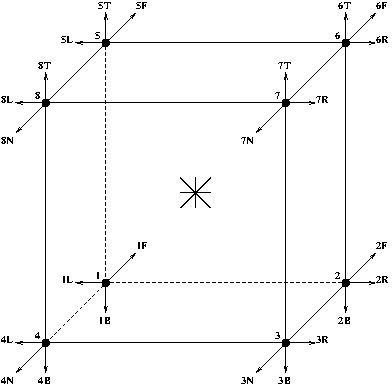
\includegraphics[width=150pt]{Figures/mesh_cell_sn}
    \caption{General mesh cell used to discretize spatial equations.}
    \label{cellmesh}
\end{figure}

First we state a few useful definitions:
%
\begin{gather*}
     \hat{\Omega} = \mu\hat{x} + \eta\hat{y} + \xi\hat{z} \\
     \iiint = \int_{z_{i - 1/2}}^{z_{i + 1/2}} \int_{y_{i - 1/2}}^{y_{i + 1/2}} \int_{x_{i - 1/2}}^{x_{i + 1/2}} \\
     dV = dxdydz \\
     \Delta_i = x_{i + 1/2 } - x_{i - 1/2} \\
     \Delta_j = y_{i + 1/2 } - y_{i - 1/2} \\
     \Delta_k = z_{i + 1/2 } - z_{i - 1/2}
\end{gather*}

Now, we integrate over the mesh cell and divide by the volume of the mesh cell ($V_c = \Delta_i\Delta_j\Delta_k$)
%
\begin{align*}
    \frac{1}{V_c}\iiint \left( \mu \frac{\partial}{\partial x} \psi(\vec{r}) + \eta \frac{\partial}{\partial x} \psi(\vec{r})  +\xi \frac{\partial}{\partial x} \psi(\vec{r})  + \Sigma_t(\vec{r}) \psi(\vec{r}) \right) dV &= \frac{1}{V_c}\iiint s(\vec{r}) dV \\
    \frac{\Delta_j\Delta_k}{V_c} \mu \int_{x_{i - 1/2}}^{x_{i + 1/2}} \partial \psi  + \frac{\Delta_i\Delta_k}{V_c} \eta \int_{y_{i - 1/2}}^{y_{i + 1/2}} \partial \psi + \frac{\Delta_i\Delta_j}{V_c} \xi \int_{z_{i - 1/2}}^{z_{i + 1/2}} \partial \psi + \Sigma_{t,i,j,k}\psi_{ijk} &= s_{ijk}  \\
    \frac{\mu}{\Delta_i} (\psi_{i+1/2} - \psi_{i-1/2} ) + \frac{\eta}{\Delta_j} (\psi_{j+1/2} - \psi_{j-1/2} ) + \frac{\xi}{\Delta_k} (\psi_{k+1/2} - \psi_{k-1/2} ) + \Sigma_{t,i,j,k}\psi_{ijk} &= s_{ijk}
\end{align*}

Now we relate the center fluxes ($\psi_{ijk}$) to the edge fluxes ($\psi_{n\pm 1/2}$) and close the above equation with a weighted average of the edge fluxes:
%
\begin{align*}
\psi_{i} &= \frac{1}{2}\bigl((1+\alpha_i)\psi_{i+1/2}+(1-\alpha_i)\psi_{i-1/2}\bigr)\\
\psi_{i+1/2} &= \frac{2}{(1+\alpha_i)}\psi_{ijk}-
    \frac{(1-\alpha_i)}{(1+\alpha_i)}\bar{\psi}_{i-1/2}\:,\quad \mu>0\:(\psi_{i-1/2}\text{ is incoming})\\
\psi_{i-1/2} &= \frac{2}{(1-\alpha_i)}\psi_{ijk}-
    \frac{(1+\alpha_i)}{(1-\alpha_i)}\bar{\psi}_{i+1/2}\:,\quad \mu<0 \:(\psi_{i+1/2}\text{ is incoming})
\end{align*}

where $-1 \leq \alpha \leq 1$ and $\bar{\psi}$ indicate the incoming flux (which will depend on $\mu$). The $\alpha$'s are weighting factors that are set to zero in the classic DD scheme ($\alpha = \pm 1$ is the step-difference scheme):
%
\begin{align*}
\psi_{i} &= \frac{1}{2}\bigl(\psi_{i+1/2}+\psi_{i-1/2}\bigr)\\
\psi_{i+1/2} &= 2\psi_{ijk} - \bar{\psi}_{i-1/2}\:,\quad \mu>0\:(\psi_{i-1/2}\text{ is incoming})\\
\psi_{i-1/2} &= 2\psi_{ijk} - \bar{\psi}_{i+1/2}\:,\quad \mu<0 \:(\psi_{i+1/2}\text{ is incoming})
\end{align*}

We substitute this into the cell balance transport equation and rearrange to arrive at the following set of equations:
%
\begin{align*}
    \psi_{ijk} &= \frac{s_{ijk} +
      \frac{2|\mu|}{\Delta i}\bar{\psi}_{i\mp1/2} +
      \frac{2|\eta|}{\Delta j}\bar{\psi}_{j\mp1/2} +
      \frac{2|\xi|}{\Delta k}\bar{\psi}_{k\mp1/2}}{
      \Sigma_{t,ijk} + \frac{2|\mu|}{\Delta i} +
      \frac{2|\eta|}{\Delta j} +
      \frac{2|\xi|}{\Delta k} }\\
    \psi_{i\pm1/2} &= 2\psi_{ijk} - \bar{\psi}_{i\mp1/2}\\
    \psi_{j\pm1/2} &= 2\psi_{ijk} - \bar{\psi}_{j\mp1/2}\\
    \psi_{k\pm1/2} &= 2\psi_{ijk} - \bar{\psi}_{k\mp1/2}
\end{align*}

for $\mu\gtrless0\:,\,\eta\gtrless0\:,\,\xi\gtrless0$. Now, in one dimension this reduces to, for $\mu\gtrless0$:
%
\begin{align*}
    \psi_{i} &= \frac{s_{i} + \frac{2|\mu|}{\Delta i}\bar{\psi}_{i\mp1/2}}{\Sigma_{t,i} + \frac{2|\mu|}{\Delta i}} \\
    \psi_{i\pm1/2} &= 2\psi_{i} - \bar{\psi}_{i\mp1/2}
\end{align*}

%
%
%

\vspace{10pt}
\begin{enumerate}[(a)]
\item for $\mu > 0$ (or moving from left to right)
\end{enumerate}

In this case, our equations become
%
\begin{align*}
\psi_{i} &= \frac{s_{i} + \frac{2\mu}{\Delta i}\bar{\psi}_{i-1/2}}{\Sigma_{t,i} + \frac{2\mu}{\Delta i}} \\
\psi_{i\pm1/2} &= 2\psi_{i} - \bar{\psi}_{i\mp1/2}
\end{align*}

Now to march through the sweeping process for one angle using the DD scheme we would first need to assume some value for the incoming flux on the left most face of our geometry. Let's number our geometry such that the first cell is $i=0$, and the next one to the right is $i=1$, and so on. So we would need to know (or be given) the incoming flux at cell 0, $\bar{\psi}_{-1/2}$. With this we can then solve for $\psi_0$ using the equation above, and then also solve for $\psi_{1/2}$ using $\bar{\psi}_{-1/2}$ and $\psi_0$. With $\psi_{1/2}$ in hand, we could then move to the next cell, $i=1$, set $\bar{\psi}_{1/2} = \psi_{1/2}$ and then solve for $\psi_1$, and then $\psi_{3/2}$. We would then repeat the process of using the left face flux to solve for the center flux, and then using the left and center fluxes together to solve for the right face flux for each cell. We do this in order, moving from the left to the right (in the direction of particle flow). Also, in each cell we are computing the source $s_i$ which very well may depend on the flux. Therefore after the sweep, we would need to update $s_i$ before starting another sweep. We continue the sweeps until we have satisfied some convergence criterion.

%
%
%

\vspace{40pt}
\begin{enumerate}[(b)]
\item for $\mu < 0$ (or moving from right to left)
\end{enumerate}

In this case, our equations become
%
\begin{align*}
\psi_{i} &= \frac{s_{i} + \frac{2|\mu|}{\Delta i}\bar{\psi}_{i+1/2}}{\Sigma_{t,i} + \frac{2|\mu|}{\Delta i}} \\
\psi_{i\pm1/2} &= 2\psi_{i} - \bar{\psi}_{i\mp1/2}
\end{align*}

The only difference now is that in order to calculate the center flux, we need to use the right face flux. Once we have the right and center fluxes, we can then solve for the left face flux. To start the sweep, we would need to assume (or be given) some value for the right-most right face flux. If we have a total of $N$ cells, then we would need to know $\bar{\psi}_{N+1/2}$. With this we would solve for $\psi_N$, and then for $\psi_{N-1/2}$ (the left face). We would then continue the process like above, but now in the opposite direction. Starting from the right most right face flux, solving for the center and left face fluxes, then moving to the next cell to the left and using the left face flux from the previous cell as the incoming flux. Again, after the sweep we update $s_i$, and then keep performing sweeps until convergence.

%
%
%

\vspace{10pt}
\begin{enumerate}[(c)]
\item at a reflecting boundary on the right edge, including how to transition from $\mu > 0$ to $\mu < 0$.
\end{enumerate}

If there was a reflecting boundary on the right most edge of the geometry, then the right moving ($\mu>0$) face flux in the right most cell will act as the left incoming flux when we switch to the $\mu < 0$ case. Using the same indexing scheme as above, the right most cell is $i=N$. We would sweep in the $\mu >0$ direction just as we did in part A (needing to be given the incoming flux on the left, $\bar{\psi}_{-1/2}$). Once we reach cell $N$, we would finish by calculating $\psi_{N+1/2}$. This flux would then be used as $\bar{\psi}_{N+1/2}$ (notice the bar) when we move into the $\mu<0$ direction and begin by solving for $\psi_N$. Once we have swept to the right AND left, we then update $s_i$ and repeat until convergence.\\

What if we have multiple angles in each direction? The above case would only work if we performed our sweep for each angle individually and the reflecting boundary reflected the particles from $\mu_1$ to $-\mu_1$. This is not always the case (some reflectors can exhibit an isotropic reflection, $\mu_1$ can reflect to $-\mu_1,\,\,-\mu_2$, etc.)

%
%
%

\vspace{10pt}
\begin{enumerate}[(d)]
\item If using the angular flux to generate flux moments during the solution process, what data do you need to store in the sweeping process?
\end{enumerate}

For each cell, we need to know the incoming flux and the source to calculate the center flux and then subsequently the outgoing flux. So we will need to store the moments of the incoming flux in order to calculate the source moments for that cell. With the incoming flux moments and source moments stored, we can calculate the center flux moments. We can then discard the source moments and use the center flux moments and incoming flux moments to calculate the outgoing flux moments. Once we have the outgoing flux moments stored, we can discard the incoming and center flux moments of that cell and then move on to the next cell, using the previous outgoing flux moments now as the incoming flux moments.\\

In each cell we need to perform three calculations - the source term, the center flux, and the outgoing flux. We do these in order and we only need the incoming flux moments to determine all three. Therefore, for each cell we only need to store the flux moments of the incoming flux into that cell. Once we move to the next cell, we can overwrite those fluxes with the incoming flux in the next cell.







% - - - - - - - - - - - - - - - - - - - - - - - - - - - - - - - - - - - - - - - - - -
\newpage
\noindent \textbf{Problem 2}\\
Let's look at truncation error in the diamond difference method by examining the 1-D case. Consider uncollided neutrons with a zero group source moving along angle $a$:
%
\begin{equation*}
\mu_a \frac{d \psi_a}{dx} + \Sigma_t \psi_a(x) = 0\:,
\end{equation*}
where the cross section is taken as constant.

\begin{enumerate}[(a)]
\item For neutrons moving $\mu_a > 0$, write an expression for the flux at some location $x'$ in terms of the flux at location $x$ (you should have an exponential).
\end{enumerate}

The differential equation above is simple enough to solve by hand. First, we rearrange:
%
\begin{align*}
    \frac{d\psi_a(x)}{dx} &= -\frac{\Sigma_t}{\mu_a } \psi_a(x) \\
    \frac{d\psi_a(x)}{\psi_a(x)} &= -\frac{\Sigma_t}{\mu_a } dx
\end{align*}

We now integrate both sides:
%
\begin{align*}
    \int \frac{d\psi_a(x)}{\psi_a(x)} &= -\frac{\Sigma_t}{\mu_a } \int dx \\
    \ln(\psi_a(x)) &= -\frac{\Sigma_t}{\mu_a }x + C \\
    \psi_a(x) &= e^{-\frac{\Sigma_t}{\mu_a }x + C} \\
    &= e^{-\frac{\Sigma_t}{\mu_a }x}e^C \\
    &= Ce^{-\frac{\Sigma_t}{\mu_a }x}
\end{align*}

Now we can write an expression for the flux at $x'$ to the flux at $x$:
%
\begin{align*}
    \frac{\psi_a(x')}{\psi_a(x)} &= \frac{e^{-\frac{\Sigma_t}{\mu_a }x'}}{e^{-\frac{\Sigma_t}{\mu_a }x}} \\
    &= e^{-\frac{\Sigma_t}{\mu_a }x'} e^{\frac{\Sigma_t}{\mu_a }x} \\
    &= e^{-\frac{\Sigma_t}{\mu_a }(x' - x)} \\
    \psi_a(x') &= \psi_a(x)e^{-\frac{\Sigma_t}{\mu_a }(x' - x)}
\end{align*}

The agrees with intuition (exponential falloff of flux into an absorbing material).

%
%
%

\vspace{10pt}
\begin{enumerate}[(b)]
\item Let's say we impose a Cartesian grid with mesh index $i$. What is the expression for $\psi_{a,i+1/2}$ in terms of $\psi_{a,i-1/2}$? Use mesh spacing $\Delta_i = x_{i+1/2} - x_{i-1/2}$ and the definition $h \equiv \frac{\Sigma_t \Delta_i}{2|\mu_a|}$.
\end{enumerate}

To gain more intuition on this problem and to relate it to part A, lets rewrite the given fluxes:
%
\begin{align*}
    \psi_{a,i+1/2} &= \psi_a(x_{i+1/2}) \\
    \psi_{a,i-1/2} &= \psi_a(x_{i-1/2})
\end{align*}

Now we see it is easy to substitute into our expression in part A:
%
\begin{align*}
     \psi_a(x_{i+1/2}) &= \psi_a(x_{i-1/2})e^{-\frac{\Sigma_t}{\mu_a }(x_{i+1/2} - x_{i-1/2})} \\
     \Rightarrow \quad \psi_{a,i+1/2} &= \psi_{a,i-1/2}\,\,e^{-\frac{\Sigma_t}{\mu_a }\Delta_i} \\
     &= \psi_{a,i-1/2}\,\,e^{-\frac{\Sigma_t}{\mu_a }\Delta_i} \\
     &= \psi_{a,i-1/2}\,\,e^{-2h} \\
\end{align*}

%
%
%

\begin{enumerate}[(c)]
\item Plug the relationship you just found into the 1D diamond difference equations ($\alpha = 0$). Manipulate those to get another expression for
 $\psi_{a,i+1/2}$ in terms of $\psi_{a,i-1/2}$ and $h$.
\end{enumerate}

The 1D DD equations are as follows:
%
\begin{align*}
    \mu_a(\psi_{a,i+1/2} - \psi_{a,i-1/2}) + \Sigma_t \Delta_i \psi_i = 0 \\
    \psi_i = \frac{1}{2}(\psi_{a,i+1/2} + \psi_{a,i-1/2})
\end{align*}

Plugging in the bottom equation into the top equation we get
%
\begin{align*}
    \psi_{a,i+1/2} - \psi_{a,i-1/2} &= -\frac{\Sigma_t \Delta_i}{2\mu_a} (\psi_{a,i+1/2} + \psi_{a,i-1/2}) \\
    \psi_{a,i+1/2} - \psi_{a,i-1/2} &= -h (\psi_{a,i+1/2} + \psi_{a,i-1/2}) \\
    \psi_{a,i+1/2}(1+h) &= \psi_{a,i-1/2}(1-h) \\
    \Rightarrow \quad \psi_{a,i+1/2} &= \left(\frac{1-h}{1+h}\right)\psi_{a,i-1/2}
\end{align*}

We did not need to plug in anything from part B... I am not sure why that was suggested.

%
%
%

\vspace{10pt}
\begin{enumerate}[(d)]
\item Look again at your solution from part b. Expand the exponential in a power series and expand your part c expression in a power series through the $h^2$ terms and show they are the same. What does that mean about the accuracy of the relationship?
\end{enumerate}

Expanding the exponential term found in part B up to the $h^2$ term, we get:
%
\begin{align*}
    e^{-2h} &\approx \frac{e^{-2h}|_{h=0}}{0!}(h-0)^0 + \frac{-2e^{-2h}|_{h=0}}{1!}(h-0)^1 + \frac{4e^{-2h}|_{h=0}}{2!}(h-0)^2 \\
    &\approx 1 - 2h + 2h^2
\end{align*}

And expanding the $\frac{1-h}{1+h}$ from part c, we get:
%
\begin{align*}
    \frac{1-h}{1+h} &\approx \frac{\frac{1-h}{1+h}|_{h=0}}{0!}(h-0)^0 + \frac{-2(1+h)^{-2}|_{h=0}}{1!}(h-0)^1 + \frac{4(1+h)^{-3}|_{h=0}}{2!}(h-0)^2 \\
    &\approx 1-2h+2h^2
\end{align*}

We see that they are the same up to $O(h^2)$ in the power series expansions. Therefore the DD scheme is a second order accurate, or $O(h^2)$, method. If we use $h$, we will get some truncation error, $\epsilon$. The second order accuracy tells us that if we use $h/2$ instead of $h$, the truncation error will be $\epsilon/4$. If we use $h/4$, the truncation error will be $\epsilon/16$, and so on.

%
%
%

\vspace{10pt}
\begin{enumerate}[(e)]
\item Look carefully at the expression for
$\psi_{a,i+1/2}$. What is a condition on $h$ that would guarantee that the flux would be positive? What does that mean about mesh spacing given the smallest $\mu_a$ in a set and a specific $\Sigma_t$?
\end{enumerate}

Inspecting the expression for $\psi_{a,i+1/2}$ in part C, we see that the resulting flux will be negative if $h>1$. Therefore to guarantee the flux to be positive, we must enforce that $h\leq1$ when using the DD scheme. It also does not make physical sense to have a negative value for $h$ (by inspection of its definition), so to be explicit, $h$ must be defined on the following domain: $0\leq h \leq 1$. Given the smallest $\mu_a$ and a specific $\Sigma_t$, the mesh spacing, $\Delta_i$, must defined to accommodate the requirement on $h$.
%
\begin{align*}
    h=\frac{\Sigma_t \Delta_i}{2|\mu_a|} \quad \Rightarrow \quad \Delta_i &= \frac{2|\mu_a| h}{\Sigma_t} = \frac{2|\mu_a| [0\rightarrow1]}{\Sigma_t} = [0 \rightarrow \frac{2|\mu_a|}{\Sigma_t}] = [0 \rightarrow 2|\mu_a| \lambda]
\end{align*}

where $\lambda$ is the mean free path in the material. Therefore we have $0 \leq \Delta_i \leq 2|\mu_a|\lambda$. Which can be very small in highly absorbing media (small mean free path) and with highly anisotropic fluxes where high order $S_N$ is needed (small minimum $|\mu_a|$ values)! With a small $\Delta_i$ (or small $h$), we have many mesh cells and thus the computation time will increase!









% - - - - - - - - - - - - - - - - - - - - - - - - - - - - - - - - - - - - - - - - - -
\newpage
\noindent \textbf{Problem 3}\\
Write a piece of code that implements the 1-D, one-speed, steady state, weighted diamond difference equations; include scattering and an external source. Use $\psi(0) = 2.0$ for $\mu > 0$; non-reentrant boundary condition at $x=0.0$ and a reflecting boundary at $x=2.0$. For this case assume isotropic scattering.\\

$\Rightarrow$ The 1-D, one-speed, steady-state, DD equations are given by:
%
\begin{align*}
    \psi_i &= \frac{s_i + \frac{2}{(1\pm\alpha_i)}\frac{|\mu|}{\Delta_i}\bar{\psi}_{i\mp1/2}}{\Sigma_{t,i} + \frac{2}{(1\pm\alpha_i)}\frac{|\mu|}{\Delta_i}}\\
    \psi_{i\pm1/2} &= \frac{2}{(1\pm\alpha_i)}\psi_{ijk}-\frac{(1\mp\alpha_i)}{(1\pm\alpha_i)}\bar{\psi}_{i\mp1/2}
\end{align*}

for $\mu\gtrless0$ and where $s_i$ includes the scattering and external source, given by:
%
\begin{align*}
    s_i &= q_{e,i} + \int_{-1}^1 d\mu' \Sigma_s(\mu'\rightarrow \mu) \psi_i(\mu') \\
    &\approx q_{e,i} + \sum_\mu w_\mu \Sigma_s \psi_i(\mu)
\end{align*}

where $q_{e,i}$ is the external source and $w_\mu$ is the quadrature weight for direction $\mu$. We are interesting in the scalar flux, which is given by:
%
\begin{align*}
    \phi &= \int_{-1}^1 d\mu \psi_i(\mu) \\
    &\approx \sum_\mu w_\mu \psi_i(\mu)
\end{align*}

%
%
%

\begin{enumerate}[(a)]
\item Explore negative flux: use the following values
\begin{itemize}
\setlength\itemsep{0em}
\item $\alpha = 0$
\item $\mu_a$ = $\pm$0.1
\item $\Sigma_t$ = 1.0
\item $\Sigma_s$ = 0
\item $q_e(x)$ = 0
\item mesh spacings: $\Delta_i = [0.08, 0.1, 0.125, 0.2, 0.4]$.
\end{itemize}
Plot the cell-centered scalar flux that results from each mesh spacing. What do you notice? How does that compare with your conclusion from the previous problem?
\end{enumerate}

$\Rightarrow$ In this case, the problem is greatly simplified. We do not need to concern ourselves with the source at all. Therefore we only need to perform one sweep (to the right and then left). Beginning with the boundary condition of $\psi(0) = 2$, we can solve for the center flux of the first mesh cell, and then subsequently the outgoing flux from that cell (all with $\mu >0$). We then set the outgoing flux as the incoming flux of the next cell and repeat for all cells until we reach the reflecting boundary at $x=2$. At this point, the outgoing flux in the $\mu>0$ direction becomes the incoming flux in the $\mu<0$ direction. We then solve for the center and outgoing flux and march through the mesh cells in the left direction. After the sweep is done, we will have an array of center flux values (angular flux). We then use our quadrature rule to integrate over direction to get the scalar flux. In this case we use an equiprobable quadrature set that is normalized to 2 (as suggested by Prof.~Slaybaugh, this will lead to cancelations later on). We only have two directions in this case, so each weight, $w_\mu$ is equal to 1.\\

The above method was implemented in Python for each mesh spacing and the code is shown below. The results of the center angular flux and center scalar flux in each mesh cell is shown in Fig.~2. The code is able to handle non-zero values of $\alpha$, therefore this same code was used for part B below. \\

\lstinputlisting[language=Python]{../p3/p3a&b.py}

\begin{figure}[H]
    \centering
    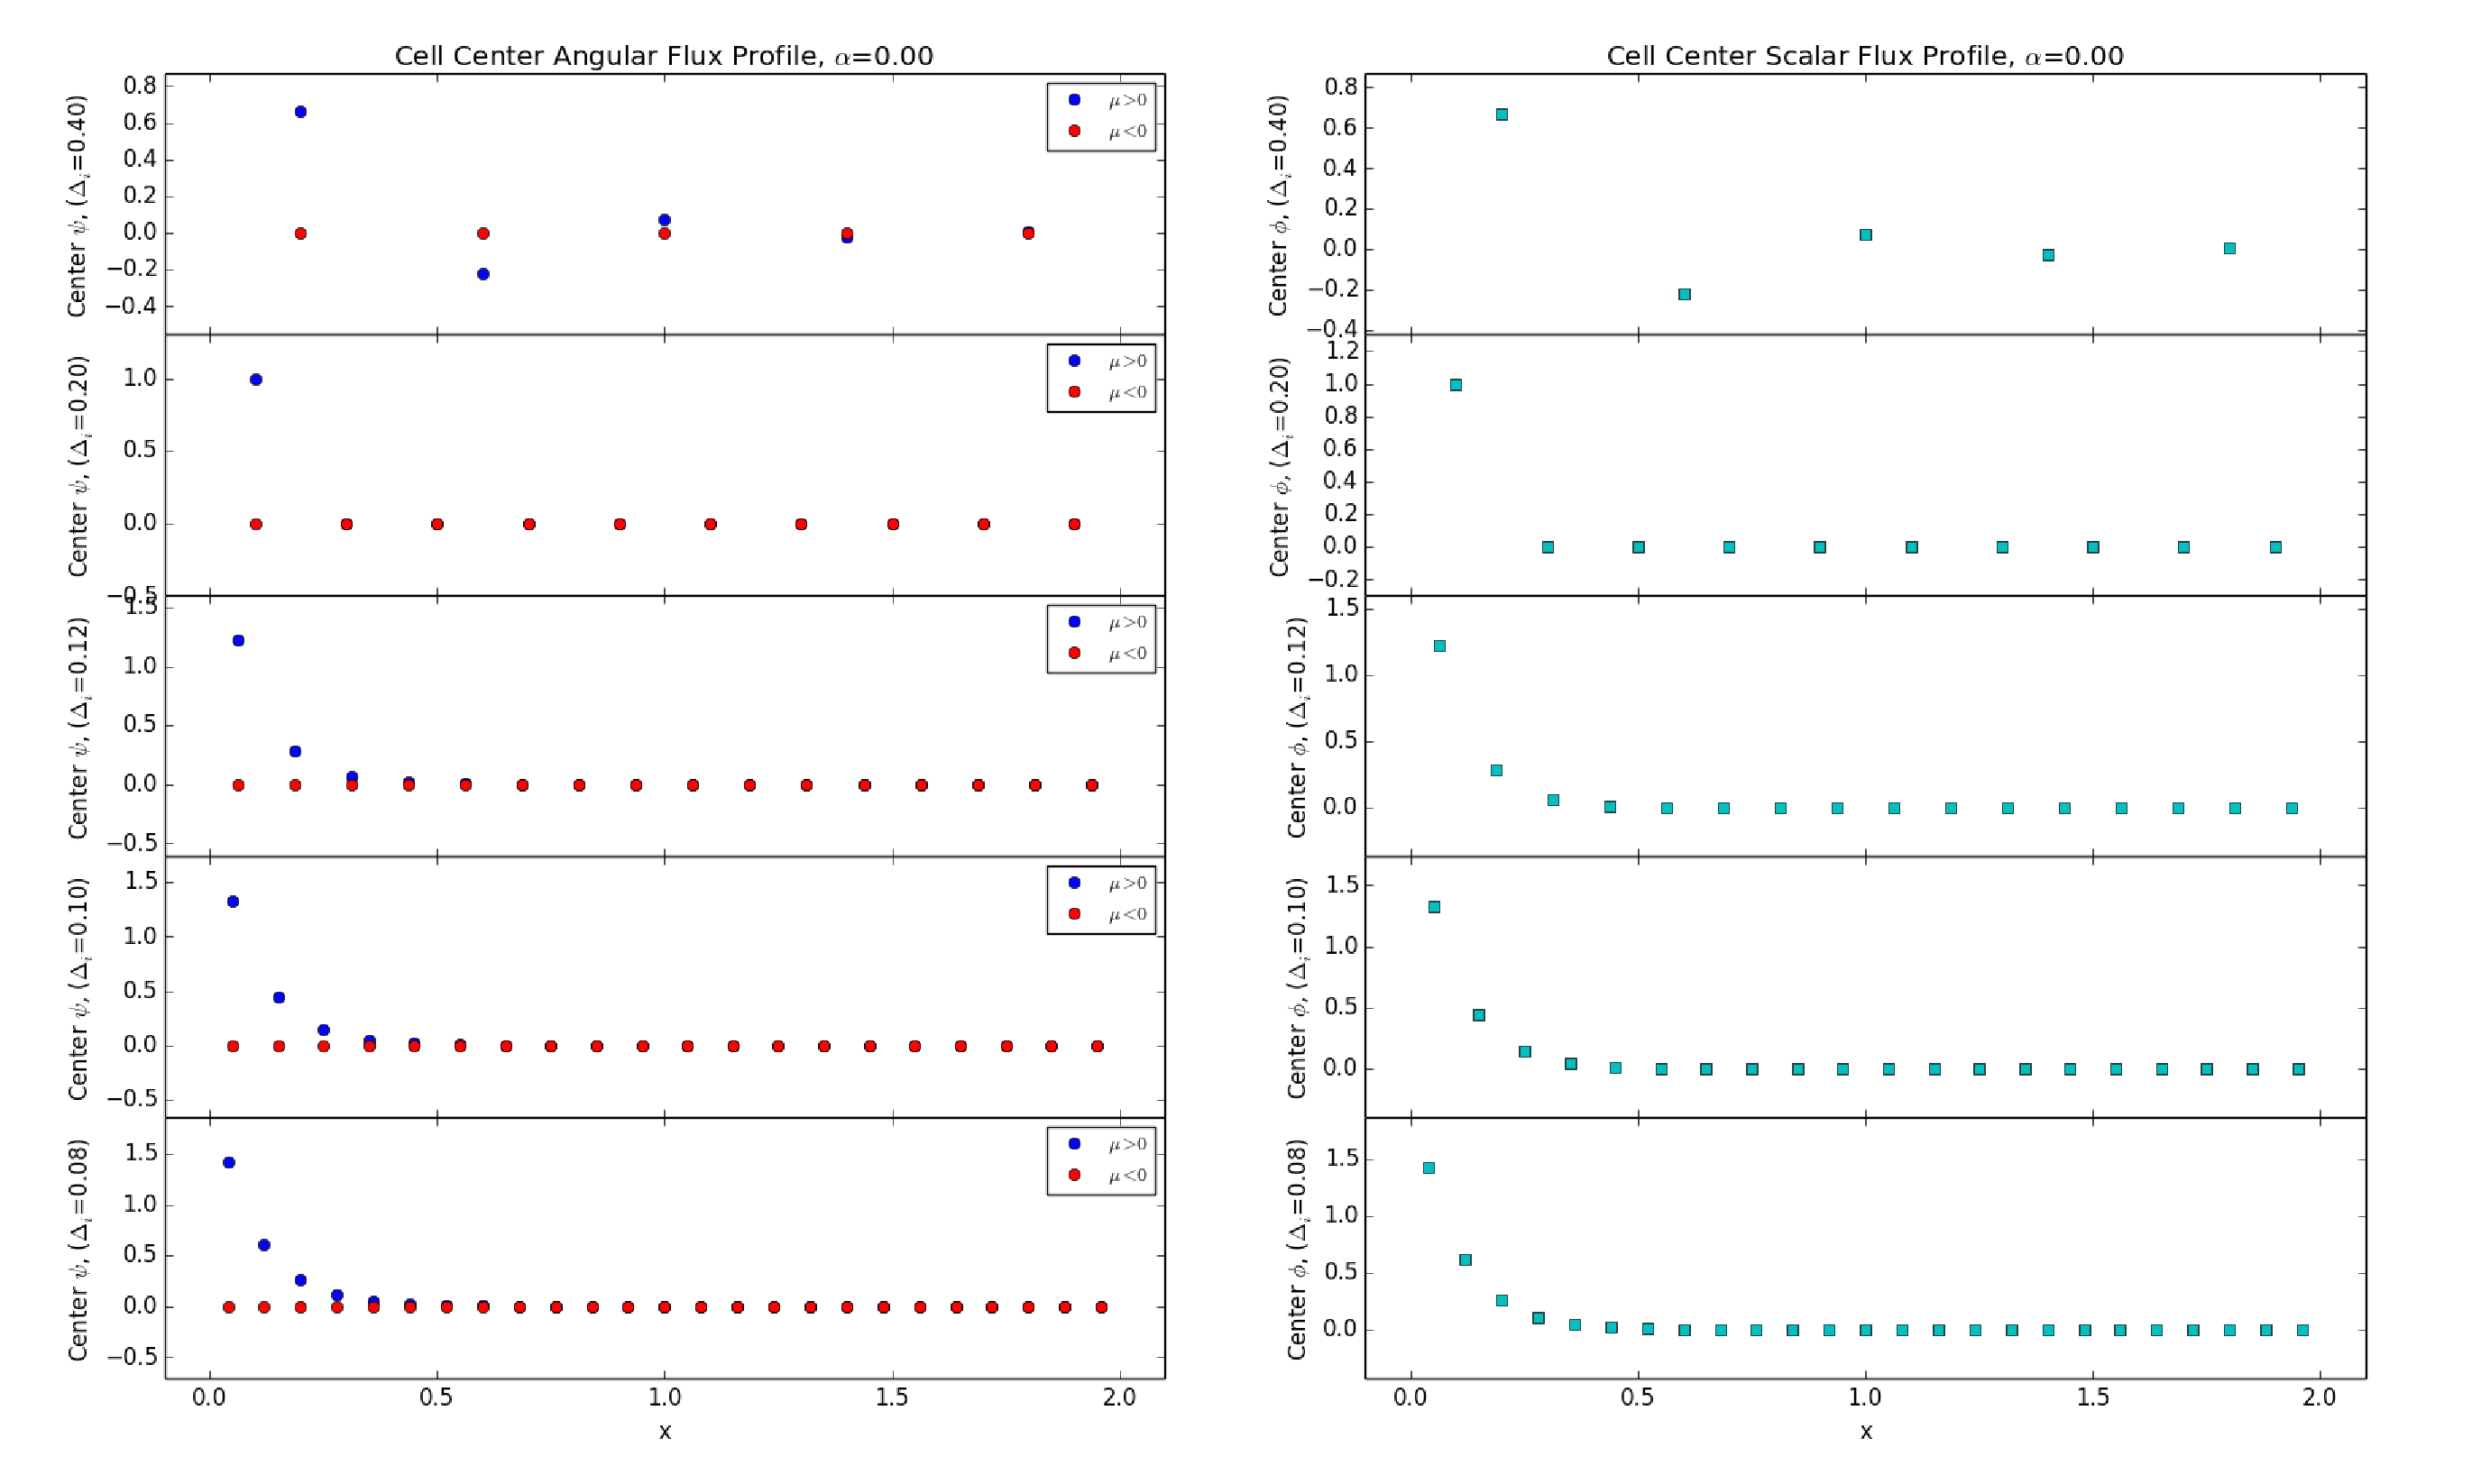
\includegraphics[width=\textwidth]{Figures/FluxProfile_a=0}
    \caption{Center angular and scalar flux profiles for varying mesh spacings with $\alpha = 0$, and no scattering or external source.}
    \label{fig2}
\end{figure}

We see that the right moving angular flux has an exponential fall off as expected. The flux is quite small by the time it reaches the reflecting boundary, so the left moving angular flux is essentially zero in all cells. In the scalar flux case, we simply add the two angular flux values together (their weights are equal to 1), and since the left moving angular flux is essentially zero, we see the scalar flux is about the same as the right moving angular flux. Now the most important thing to notice is that the flux (in both angular and scalar) goes negative in the $\Delta_i = 0.4$ case. In the previous problem, we derived that $\Delta_i$ must be less than or equal to $\frac{2|\mu|}{\Sigma_t}$ to avoid negative flux, which in this case is equal to 0.2. This is violated  when $\Delta_i = 0.4$, and thus our calculation indeed results in a negative flux value. This agrees with our conclusion from the previous problem.

%
%
%

\vspace{10pt}
\begin{enumerate}[(b)]
\item Impact of $\alpha$: try $\alpha = [-0.9, -0.5, 0.25, 0.5, 0.9]$. What happens?
\end{enumerate}

We use the same code as above, but we now vary $\alpha$. The results are shown in Figs.~3-7. \\

For $\alpha=-0.9$, we observe positive and negative fluxes for mesh spacings greater than 0.1. For a mesh spacing of 0.1, the flux seems to drop off rather quickly near the left boundary. The smallest mesh spacing (0.08) seems to produce a reasonable looking flux. For $\alpha=-0.5$, we again observe positive and negative fluxes, but now only for mesh spacings greater than 0.12. The flux also exhibits the quick exponential fall-off for mesh spacing smaller than 0.12, but it begins to look more reasonable as the mesh spacing is decreased further. For $\alpha=0.25$, only a mesh spacing of 0.4 produces negative flux values. And again, the flux begins to look more reasonable as the mesh spacing is decreased further. For $\alpha=0.5$, we no longer have any negative fluxes and the flux looks more reasonable as the mesh spacing is decreased (only have a quick fall off for a mesh spacing of 0.4). For $\alpha=0.9$, we no longer have any negative fluxes and the flux looks more reasonable as the mesh spacing is decreased (it also looks smoother than $\alpha=0.5$ for all mesh spacings).\\

It seems that as we increase the value of $\alpha$, we start to improve the behavior for large mesh spacings. This is good because in the instance where large meshing is needed (to reduce computational time), we can introduce a large positive value of $\alpha$ to assist in better reconstructing the flux (at least for the parameters we are using here).

\begin{figure}[H]
    \centering
    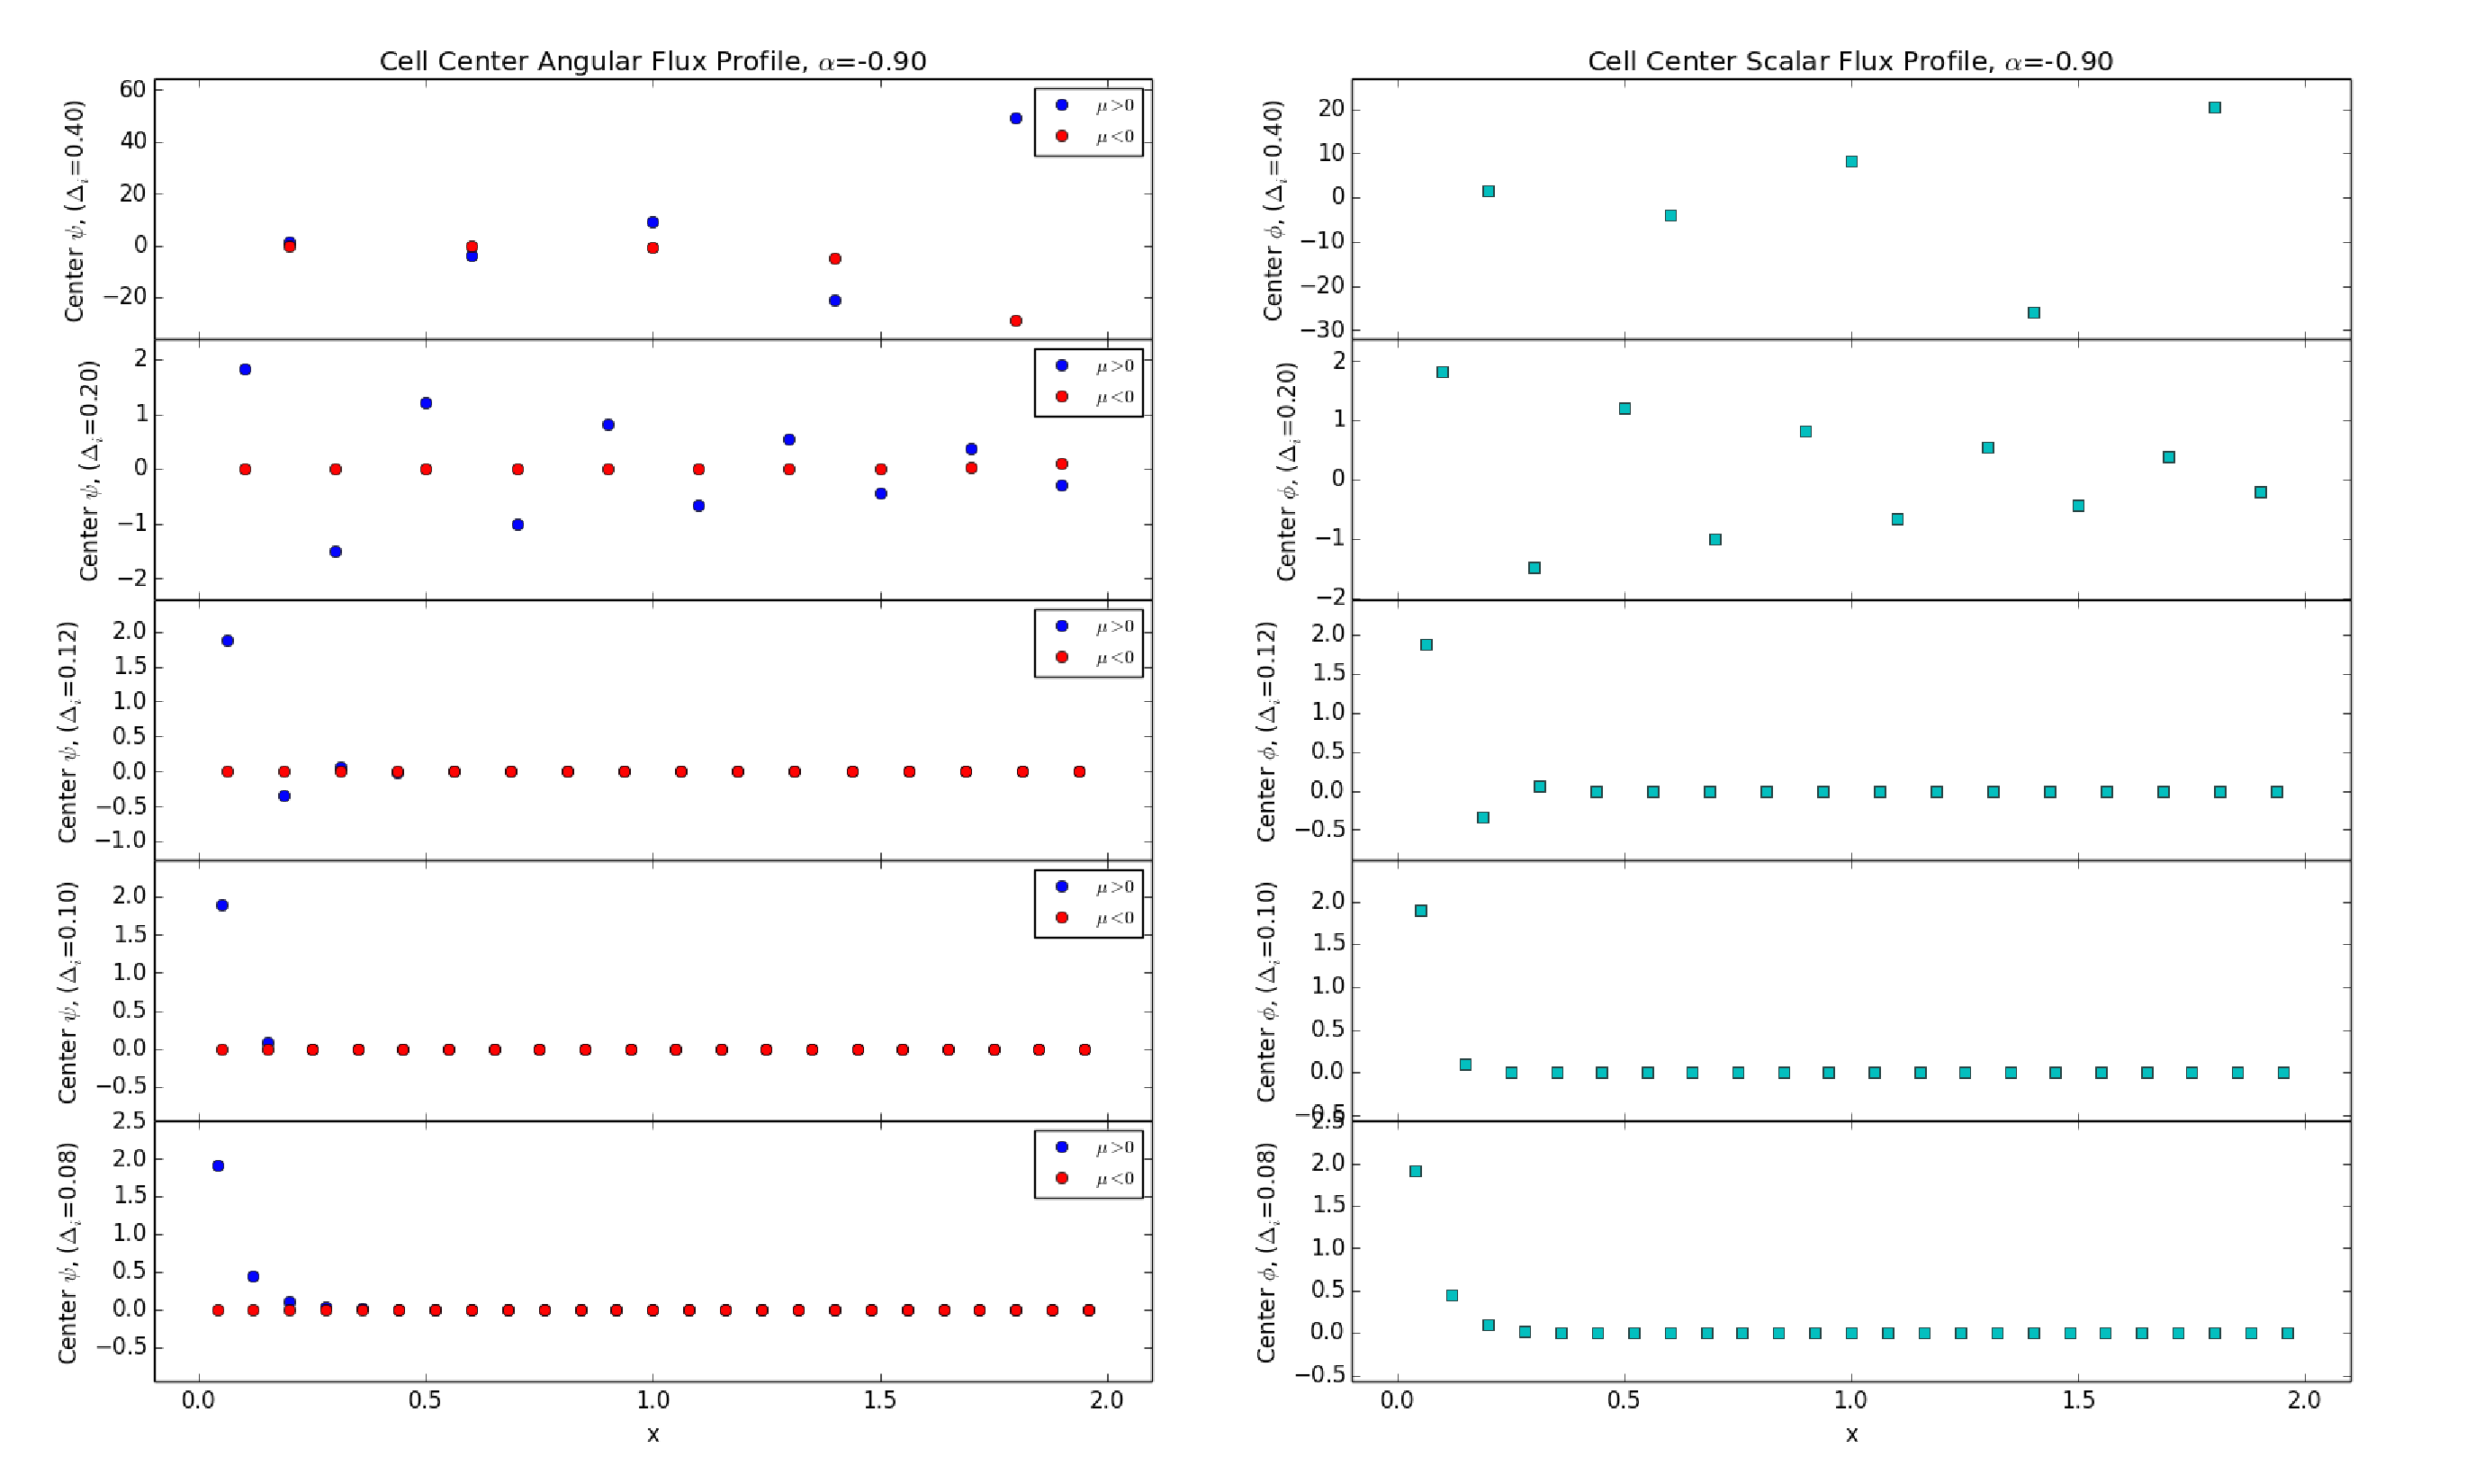
\includegraphics[width=0.9\textwidth]{Figures/FluxProfile_a=-09}
    \caption{Center angular and scalar flux profiles for varying mesh spacings with $\alpha = -0.9$, and no scattering or external source.}
    \label{fig3}
\end{figure}

\begin{figure}[H]
    \centering
    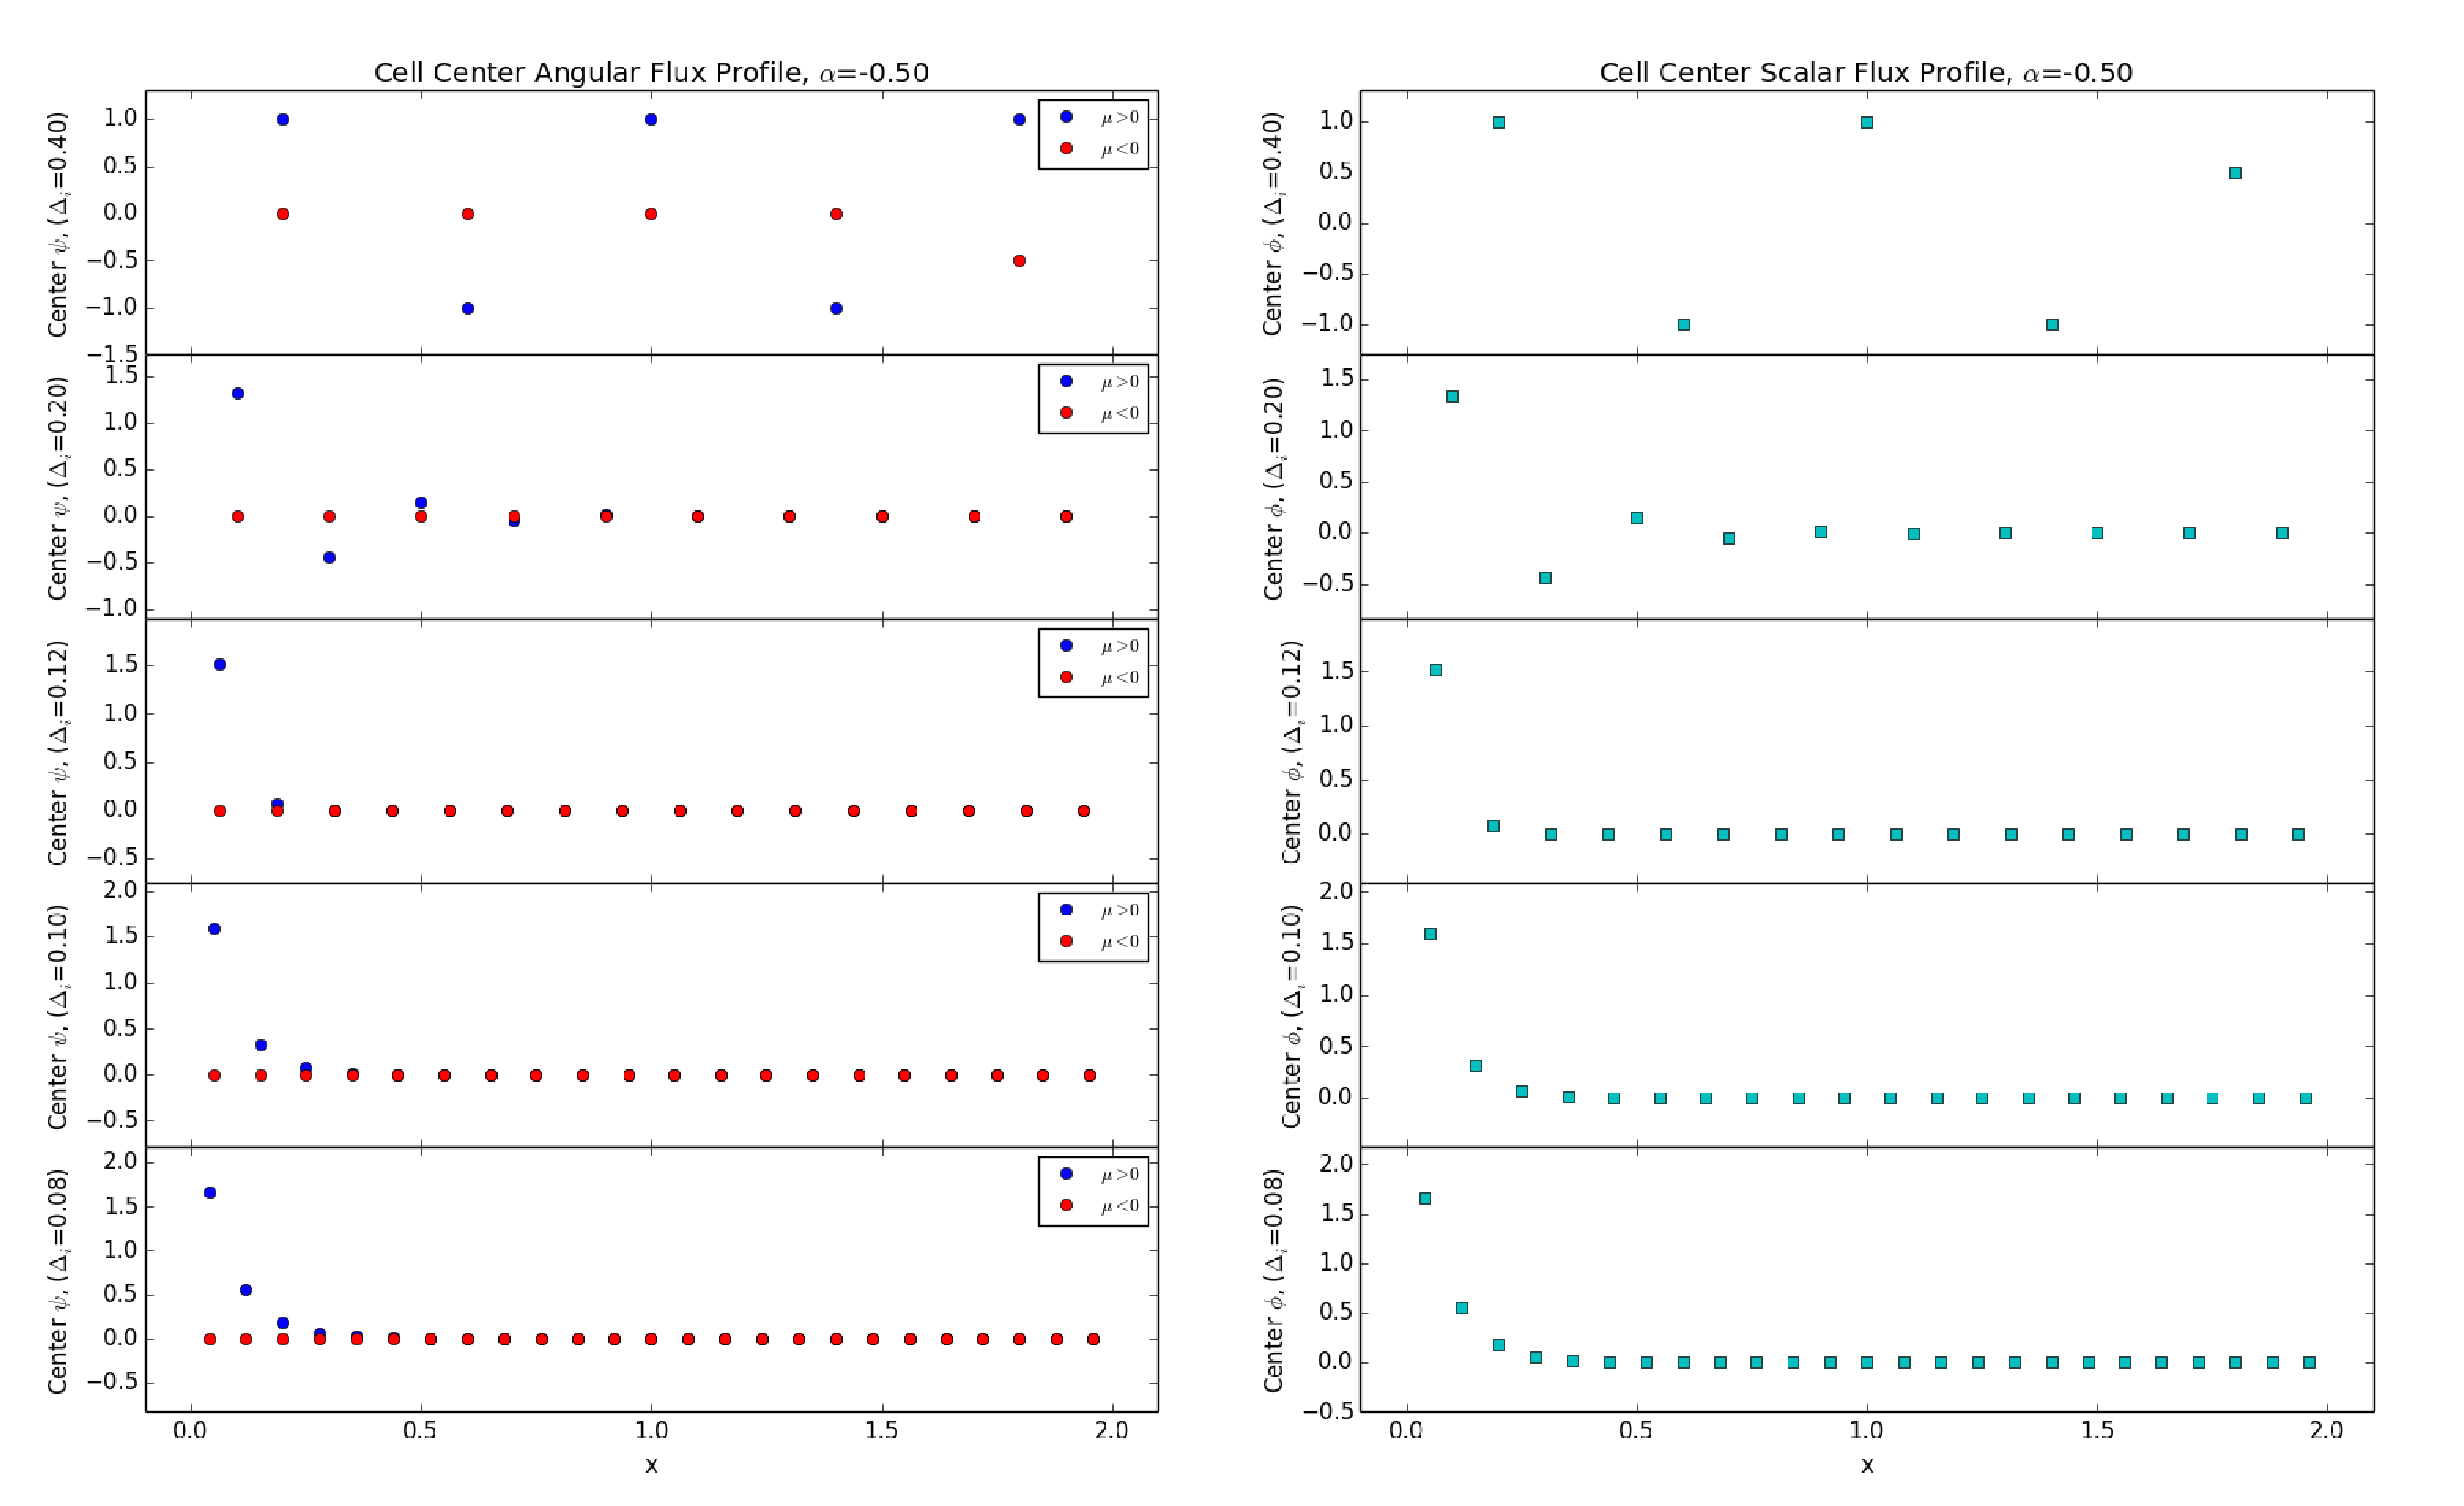
\includegraphics[width=0.9\textwidth]{Figures/FluxProfile_a=-05}
    \caption{Center angular and scalar flux profiles for varying mesh spacings with $\alpha = -0.5$, and no scattering or external source.}
    \label{fig4}
\end{figure}

\begin{figure}[H]
    \centering
    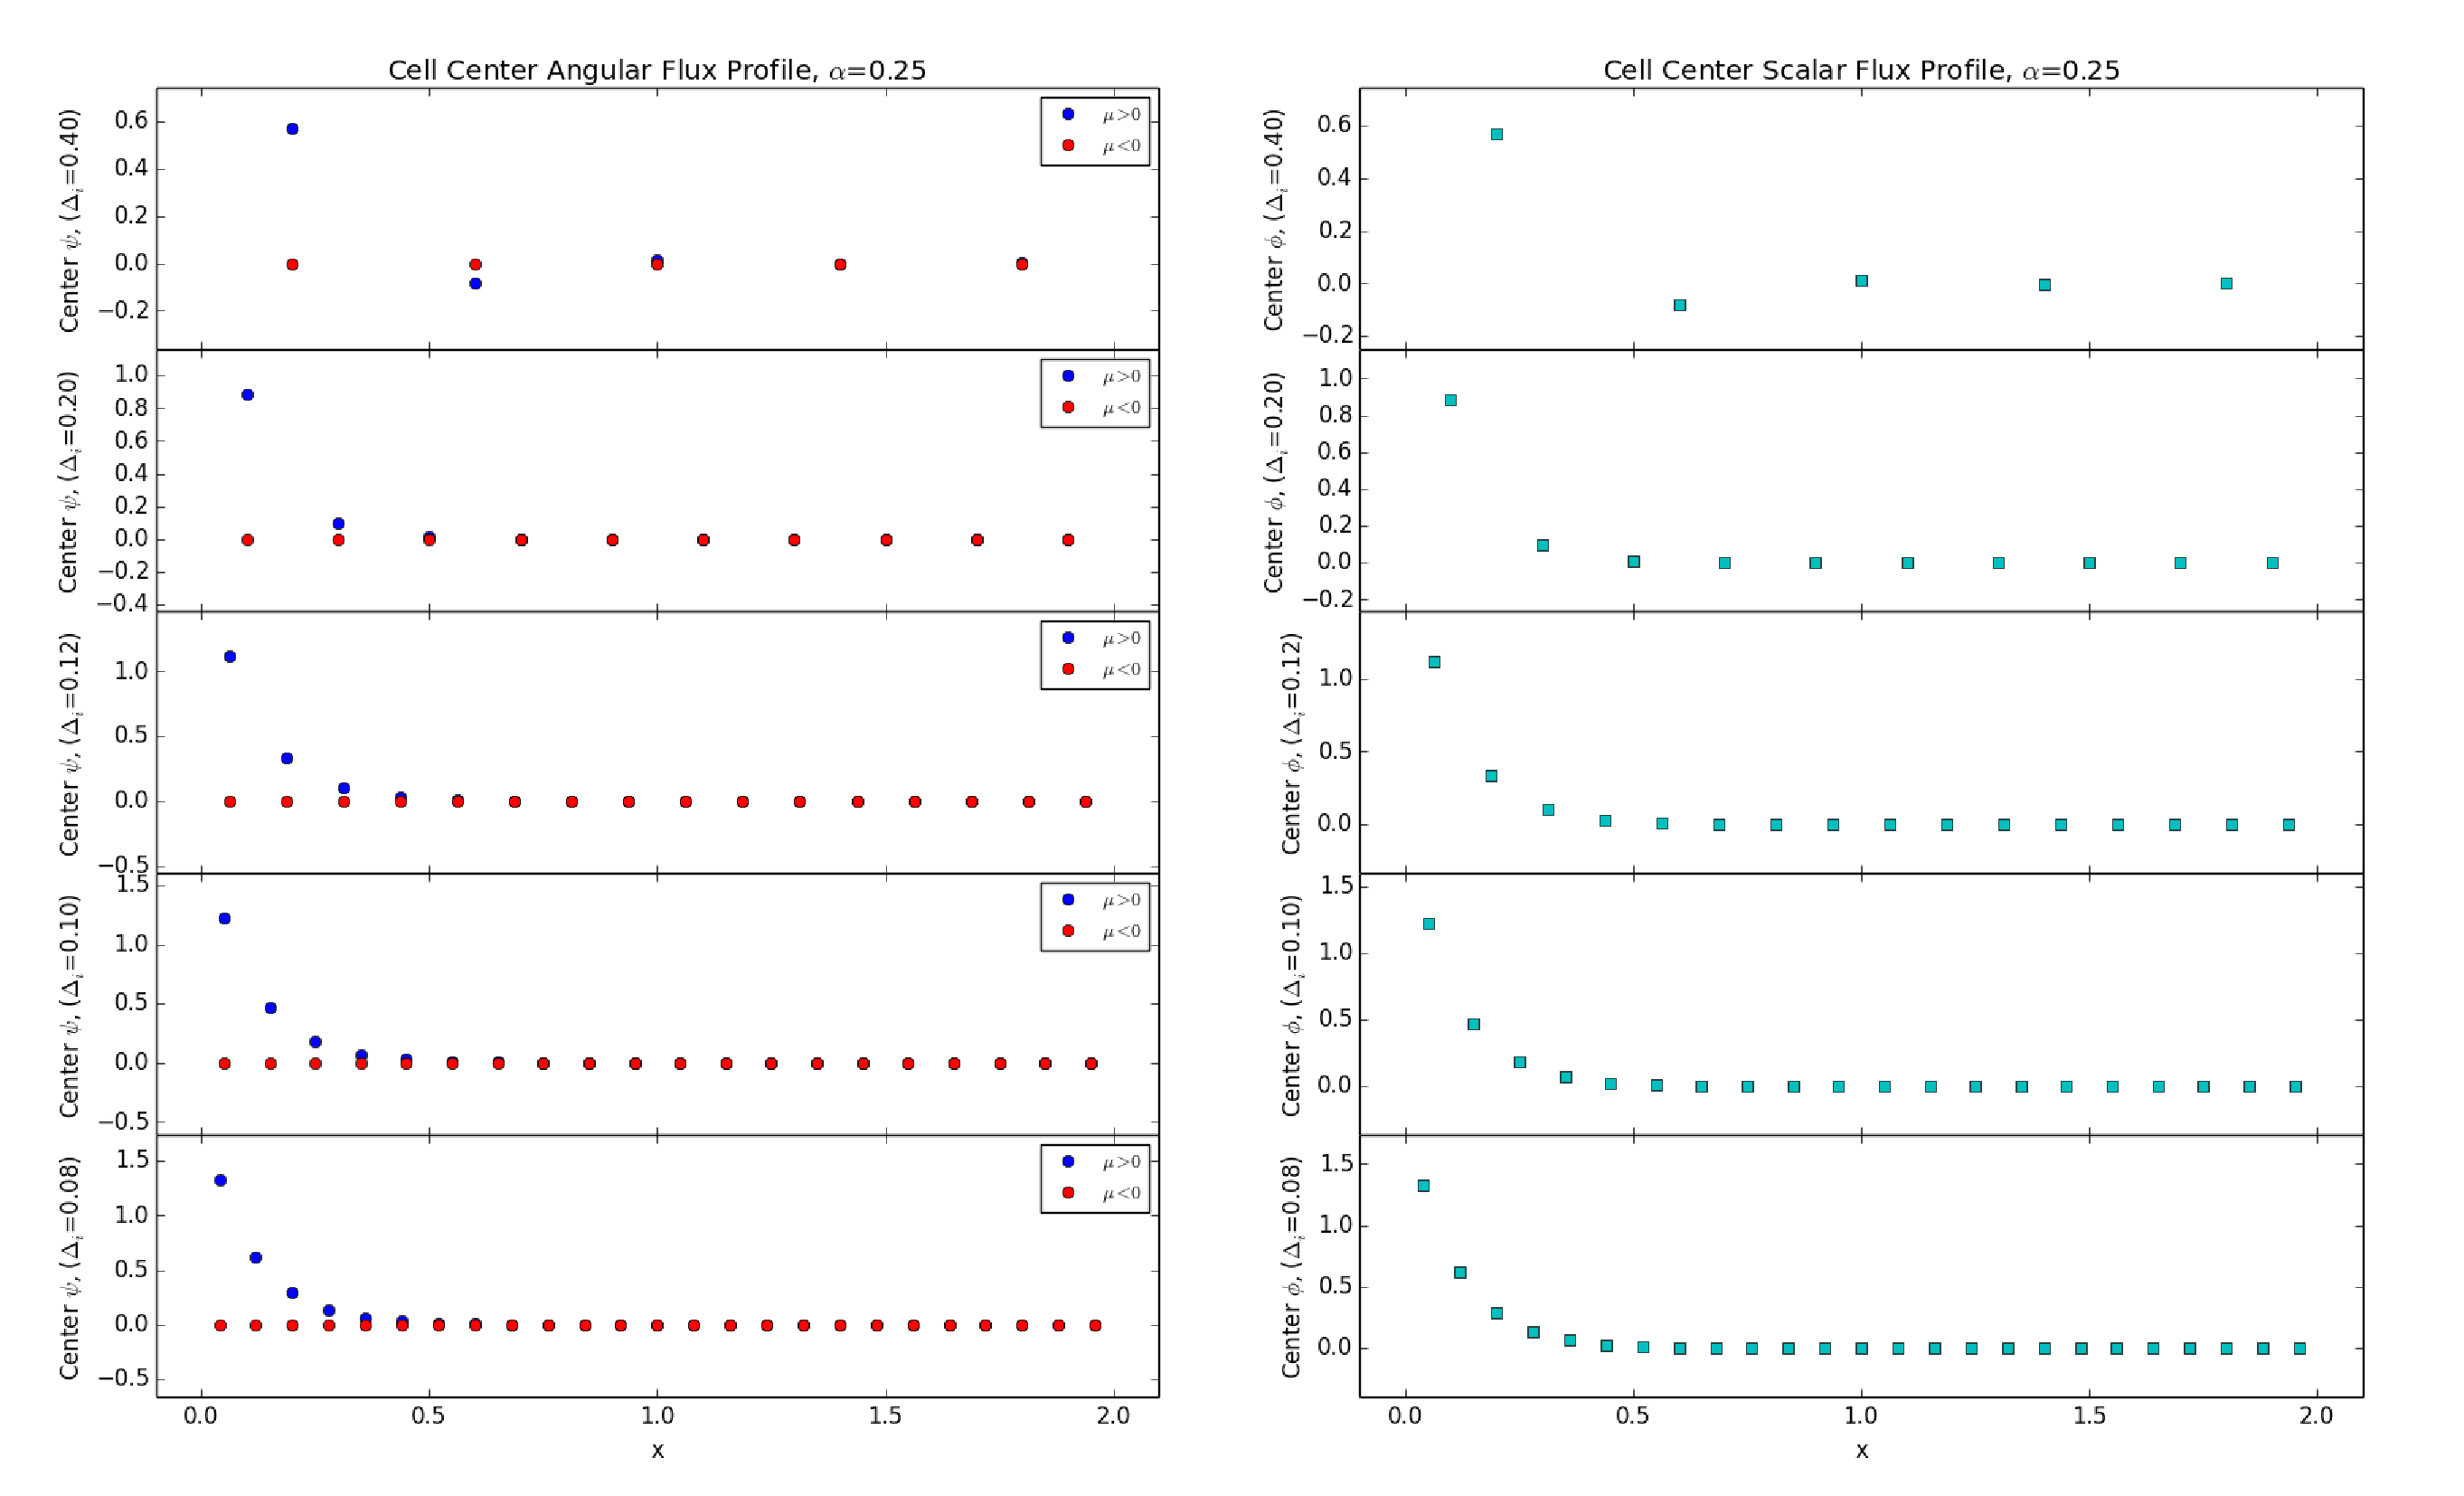
\includegraphics[width=0.9\textwidth]{Figures/FluxProfile_a=025}
    \caption{Center angular and scalar flux profiles for varying mesh spacings with $\alpha = 0.25$, and no scattering or external source.}
    \label{fig5}
\end{figure}

\begin{figure}[H]
    \centering
    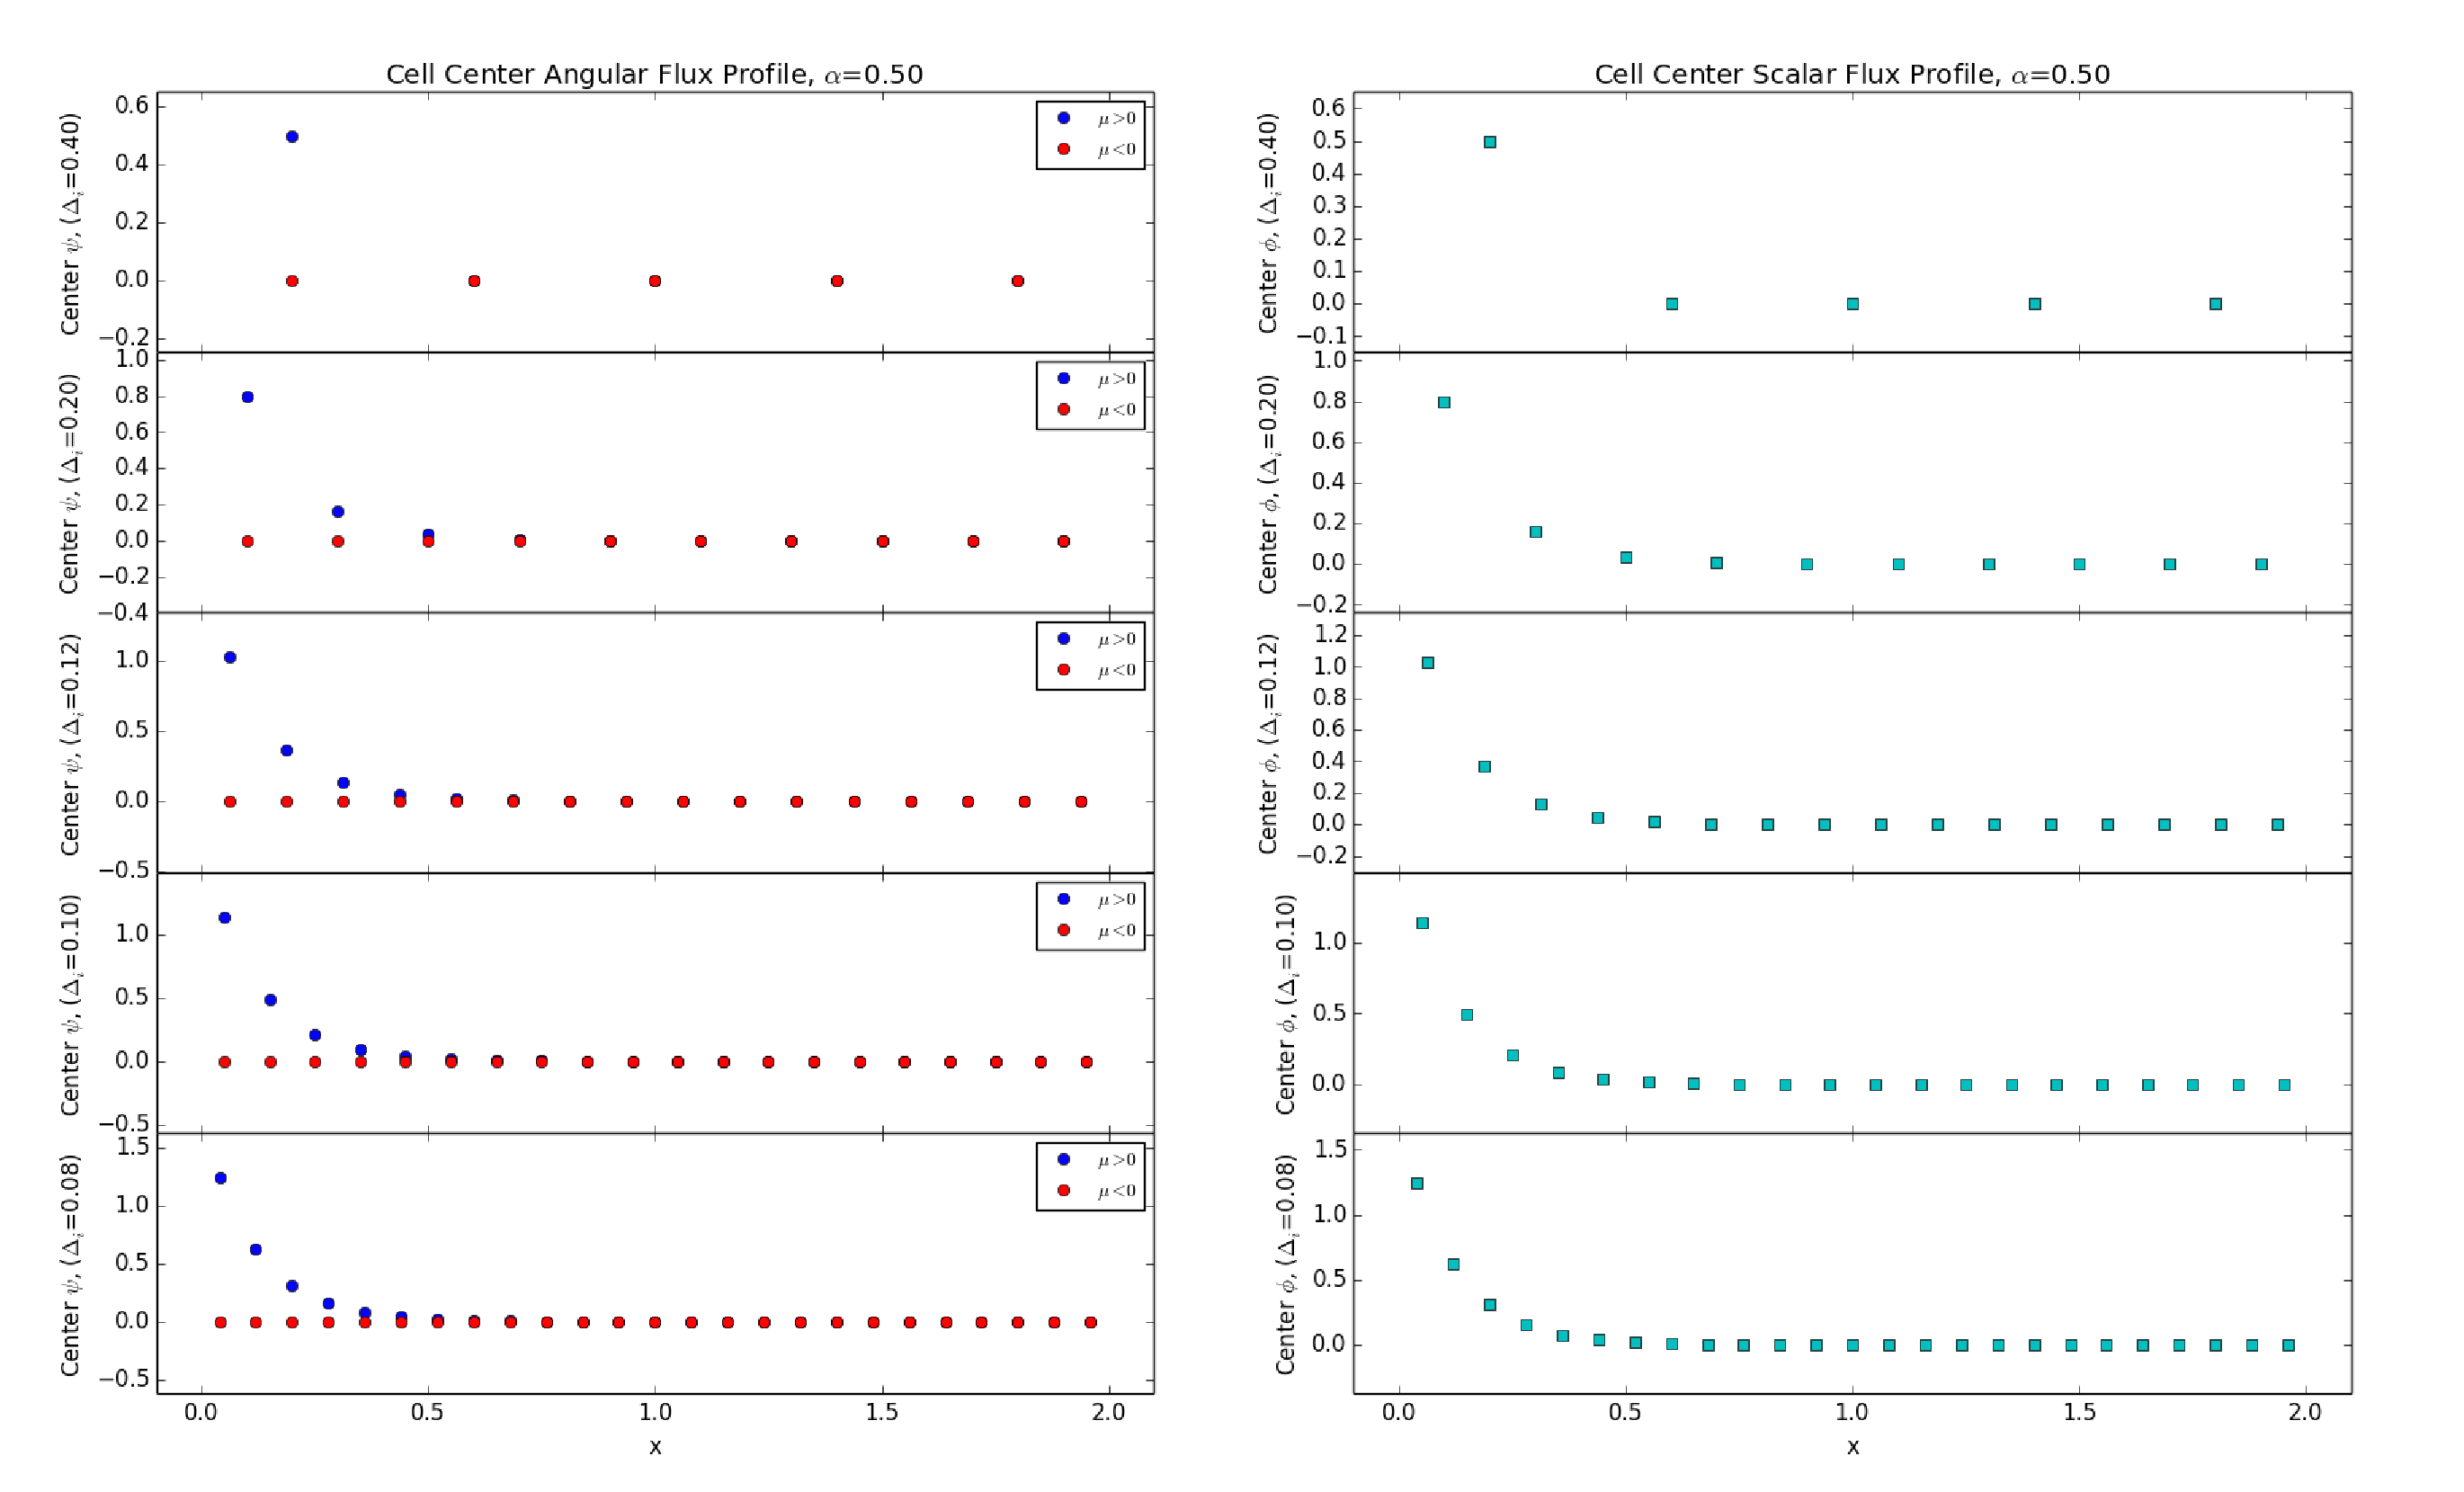
\includegraphics[width=0.9\textwidth]{Figures/FluxProfile_a=05}
    \caption{Center angular and scalar flux profiles for varying mesh spacings with $\alpha = 0.5$, and no scattering or external source.}
    \label{fig6}
\end{figure}

\begin{figure}[H]
    \centering
    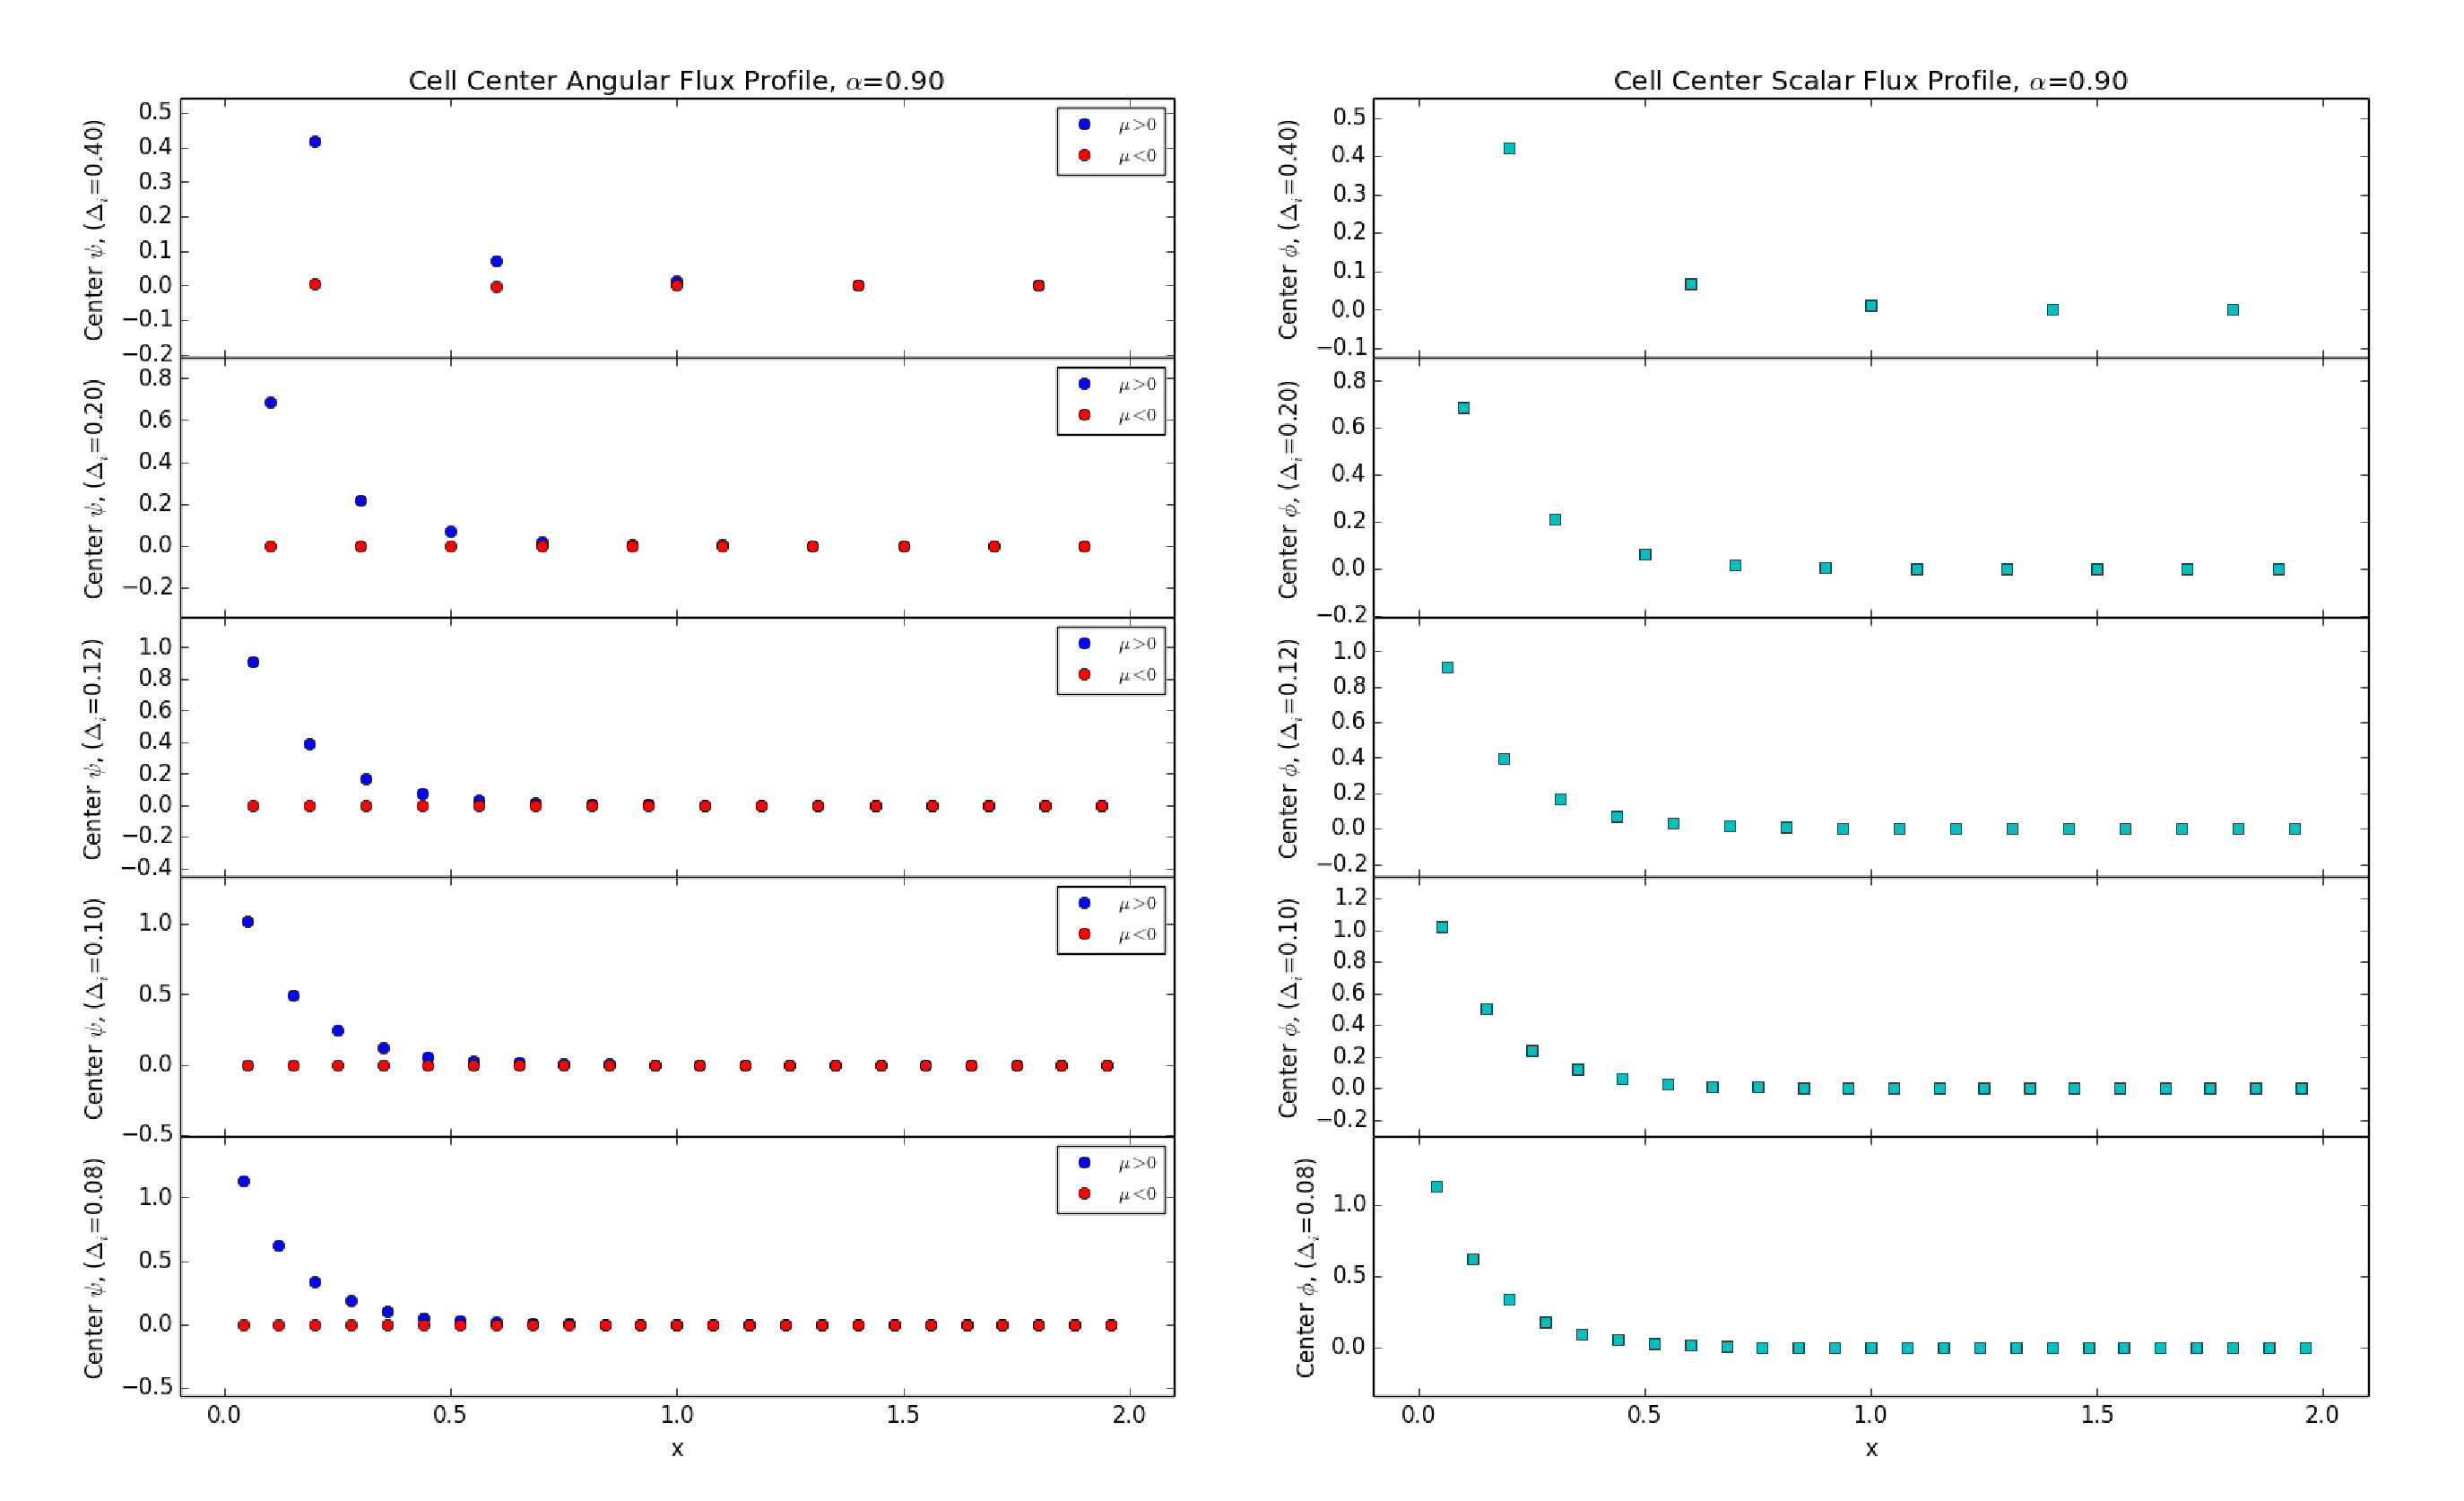
\includegraphics[width=0.9\textwidth]{Figures/FluxProfile_a=09}
    \caption{Center angular and scalar flux profiles for varying mesh spacings with $\alpha = 0.9$, and no scattering or external source.}
    \label{fig7}
\end{figure}

%
%
%

\begin{enumerate}[(c)]
\item Real results? Now try adding a source
\begin{itemize}
\setlength\itemsep{0em}
\item $\alpha = [-0.5, 0, 0.5]$ (feel free to try others)
\item $\mu$ = $\pm$[0.2, 0.7] %(use 0.2 for the $\alpha$ studies and then choose one $alpha$ to use with 3 angles); for simplicity just use equiprobable weights to get scalar flux from angular flux (note: this is not a real quadrature set)
\item $\Sigma_t$ = 1.0
\item $\Sigma_s$ = 0.5
\item $q_e(x)$ = 1.0
\end{itemize}
Report the results.
\end{enumerate}

Now we wish to include scattering, an external source, and more angles. Let's first consider scattering. We can use the quadrature to evaluate the integral over angle, but now we have 4 angles and thus to keep the same normalization as before (= 2), each equiprobable weight will now be 0.5. Therefore our scattering source in each mesh cell $i$ will be given by
%
\begin{align*}
    \sum_\mu w_\mu \Sigma_s \psi_i(\mu) = \frac{\Sigma_s}{2}\left[\psi_i(-0.7) + \psi_i(-0.2) + \psi_i(0.2) + \psi_i(0.7)\right]
\end{align*}

In each sweep we now calculate $s_i$ and we also now calculate the angular flux for both angles (in both directions). We will need to assume some initial values of the angular flux when we first calculate the scattering source (I will assume a value of 1 in all cells and all directions). Once we do a full sweep (right and left), we then update the source term with the newly calculated angular flux values. After each sweep (right and left) we also calculate the scalar flux with our new quadrature weights. As we iterate through the sweeps and update the flux, we need to define a convergence criterion to eventually stop our calculation. My first attempt is to use the $l_2$ norm of the difference between the current scalar flux and the previous scalar flux. Once we have satisfied:
%
\begin{align*}
    || \phi^k - \phi^{k-1} ||_{l_2} < 10^{-4}
\end{align*}

we stop the calculation and plot the results. The modified code is shown below, and the results using the three different values of $\alpha$ are shown in Figs.~8-10.

\lstinputlisting[language=Python]{../p3/p3c&d.py}

\begin{figure}[H]
    \centering
    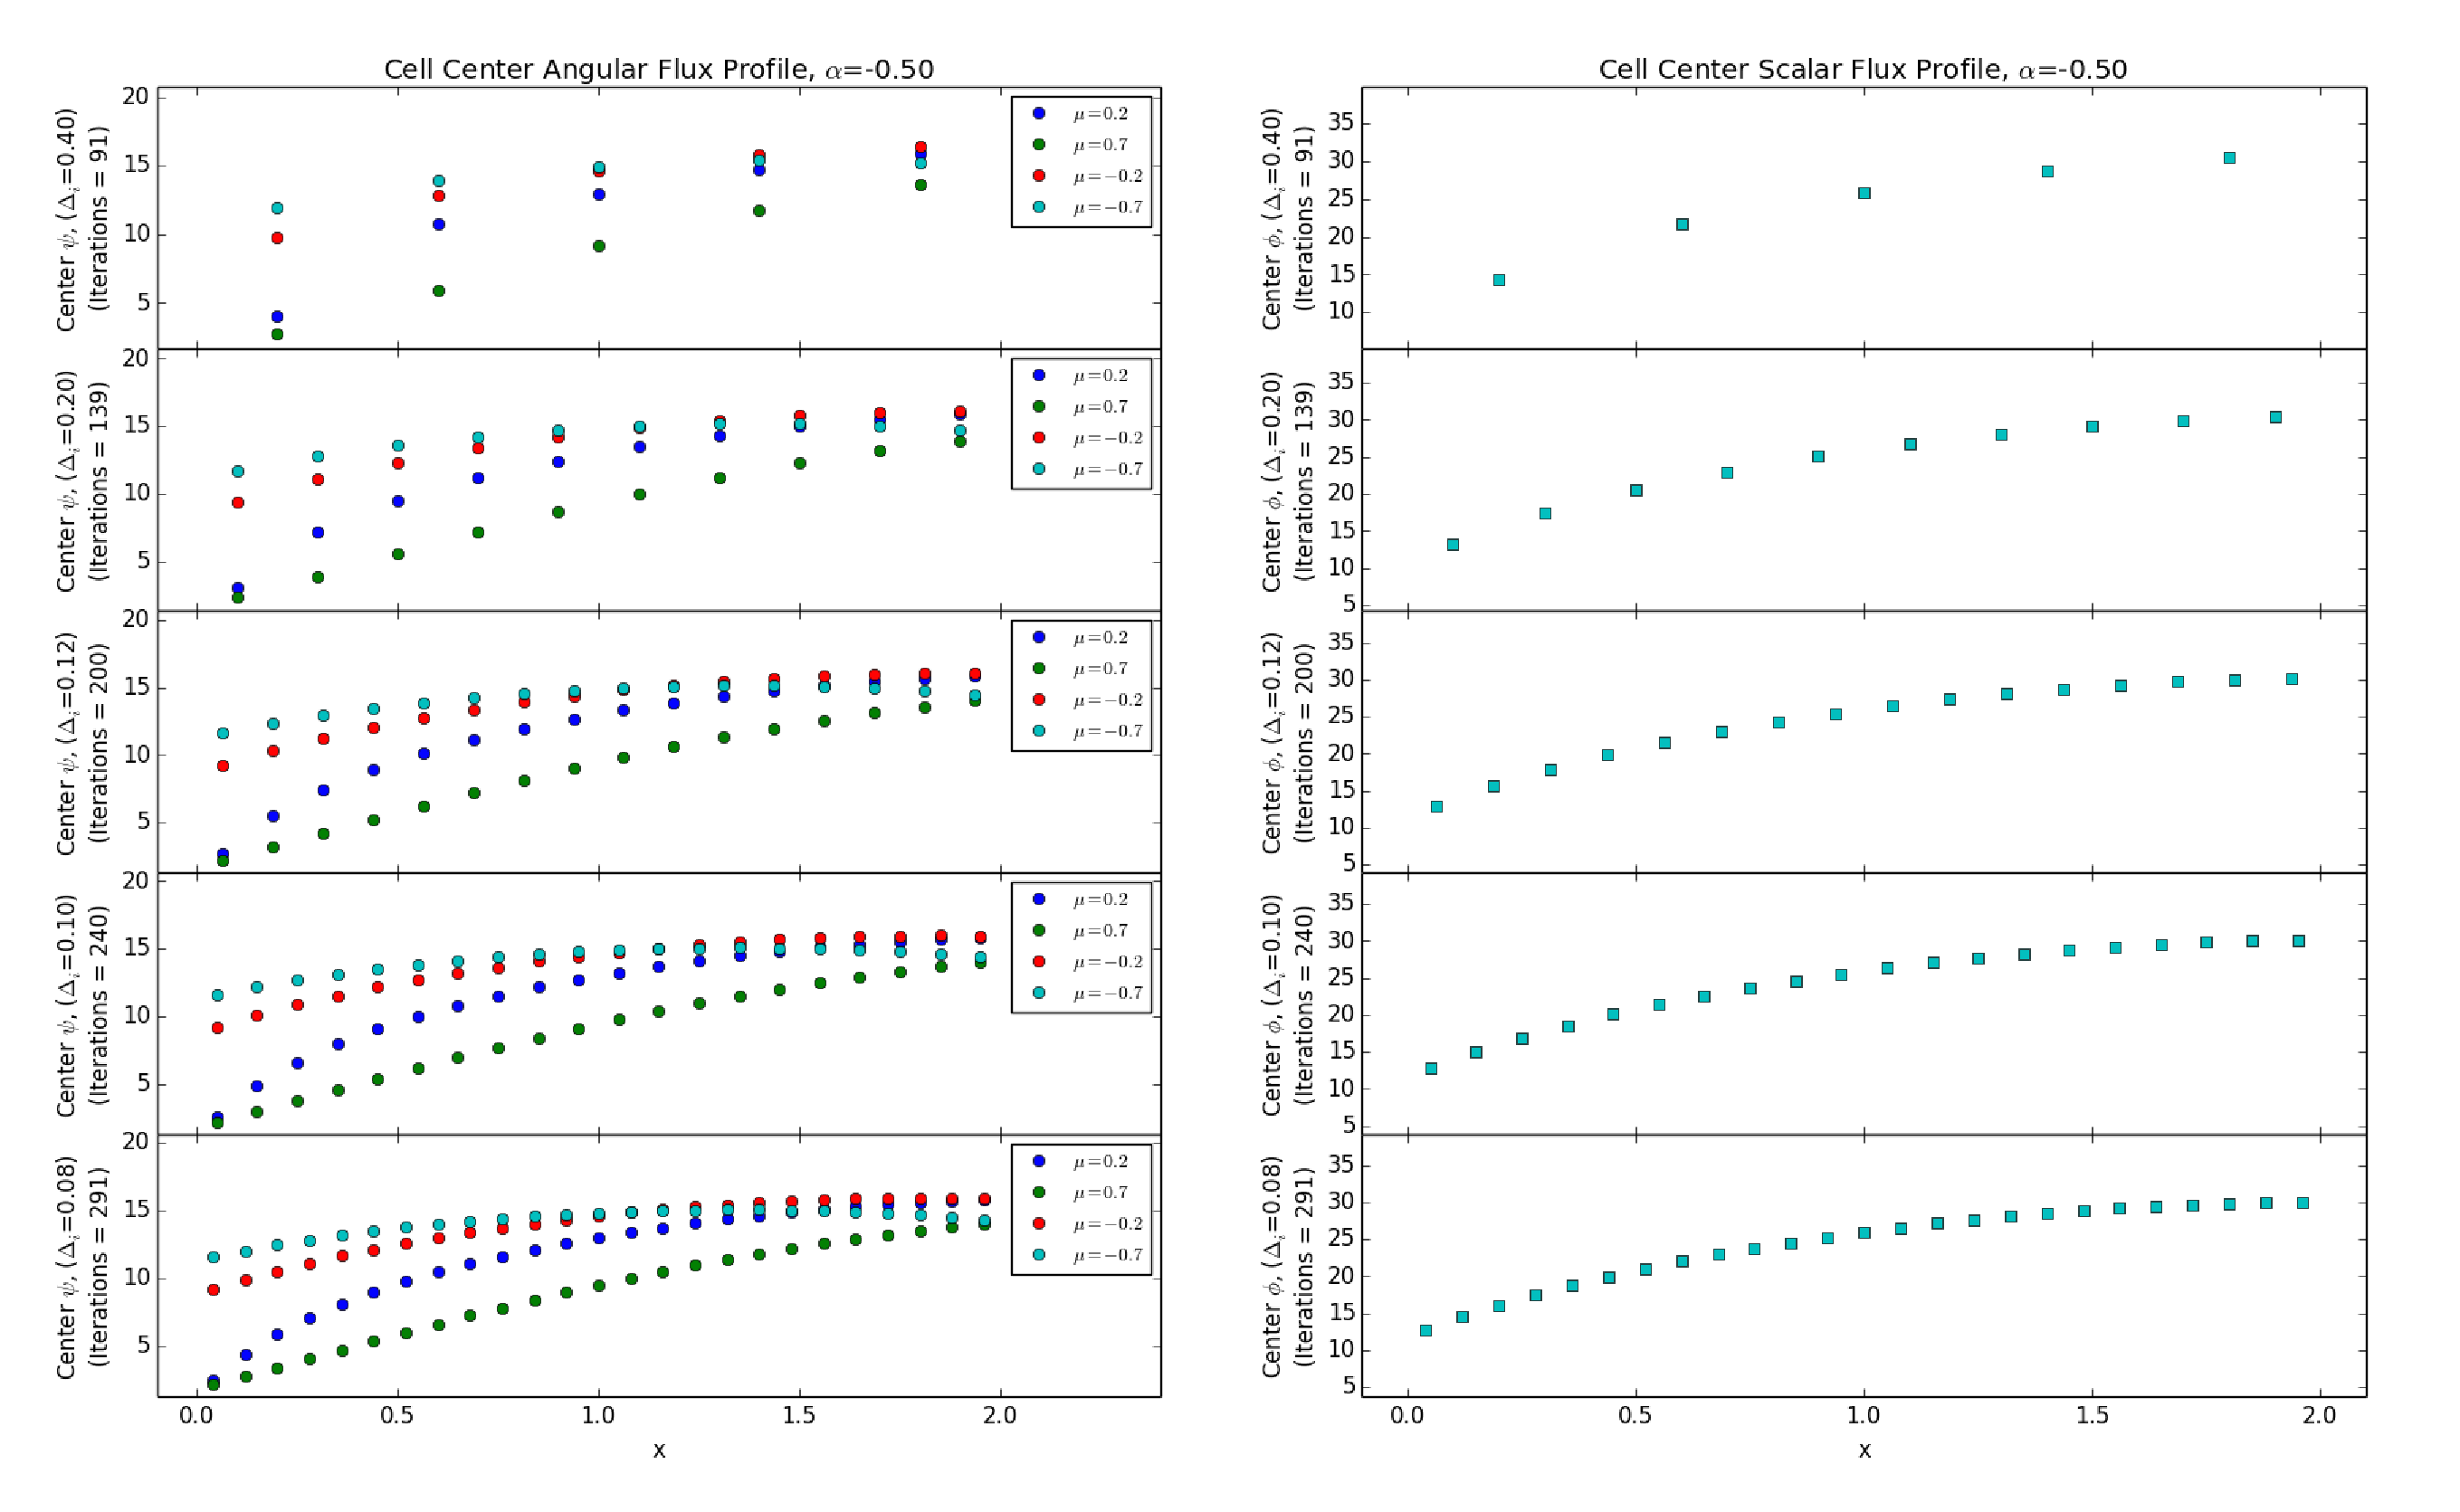
\includegraphics[width=0.9\textwidth]{Figures/FluxProfile_a=-05_source}
    \caption{Center angular and scalar flux profiles for varying mesh spacings with $\alpha = -0.5$, with scattering ($\Sigma_s = 0.5$) and external source ($q_e=1$).}
    \label{fig8}
\end{figure}

\begin{figure}[H]
    \centering
    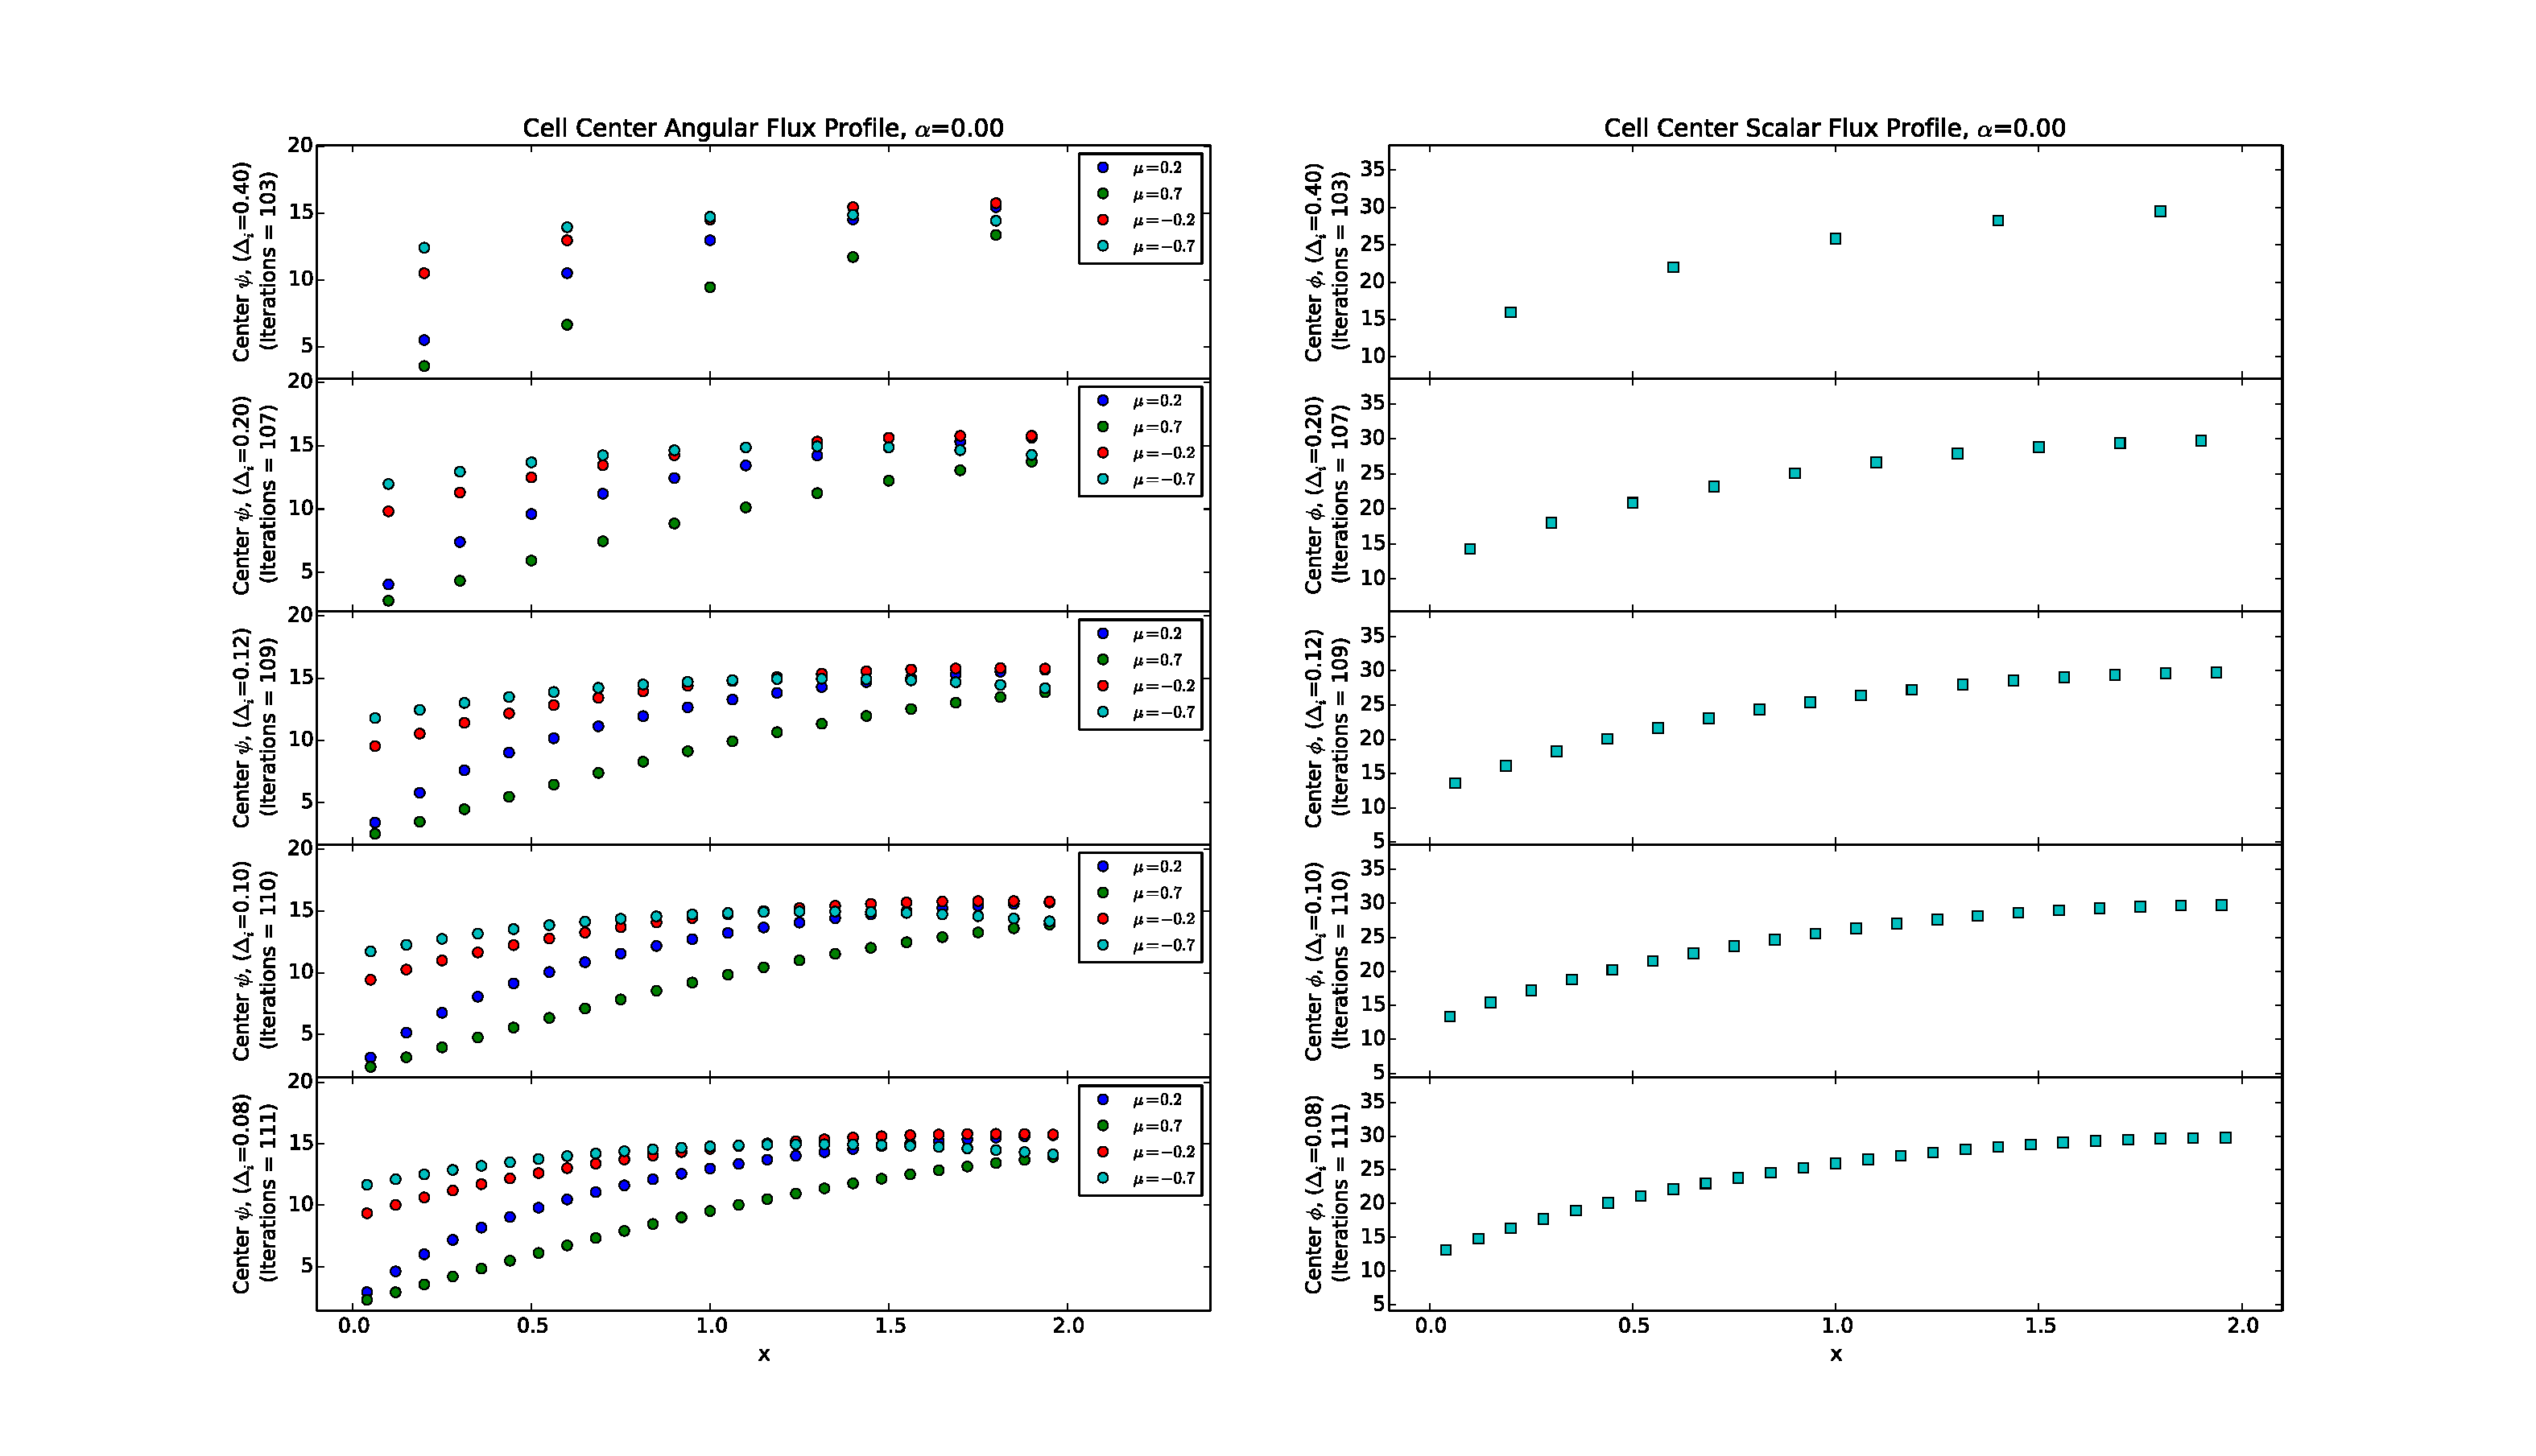
\includegraphics[width=0.9\textwidth]{Figures/FluxProfile_a=0_source}
    \caption{Center angular and scalar flux profiles for varying mesh spacings with $\alpha = 0$, with scattering ($\Sigma_s = 0.5$) and external source ($q_e=1$).}
    \label{fig9}
\end{figure}

\begin{figure}[H]
    \centering
    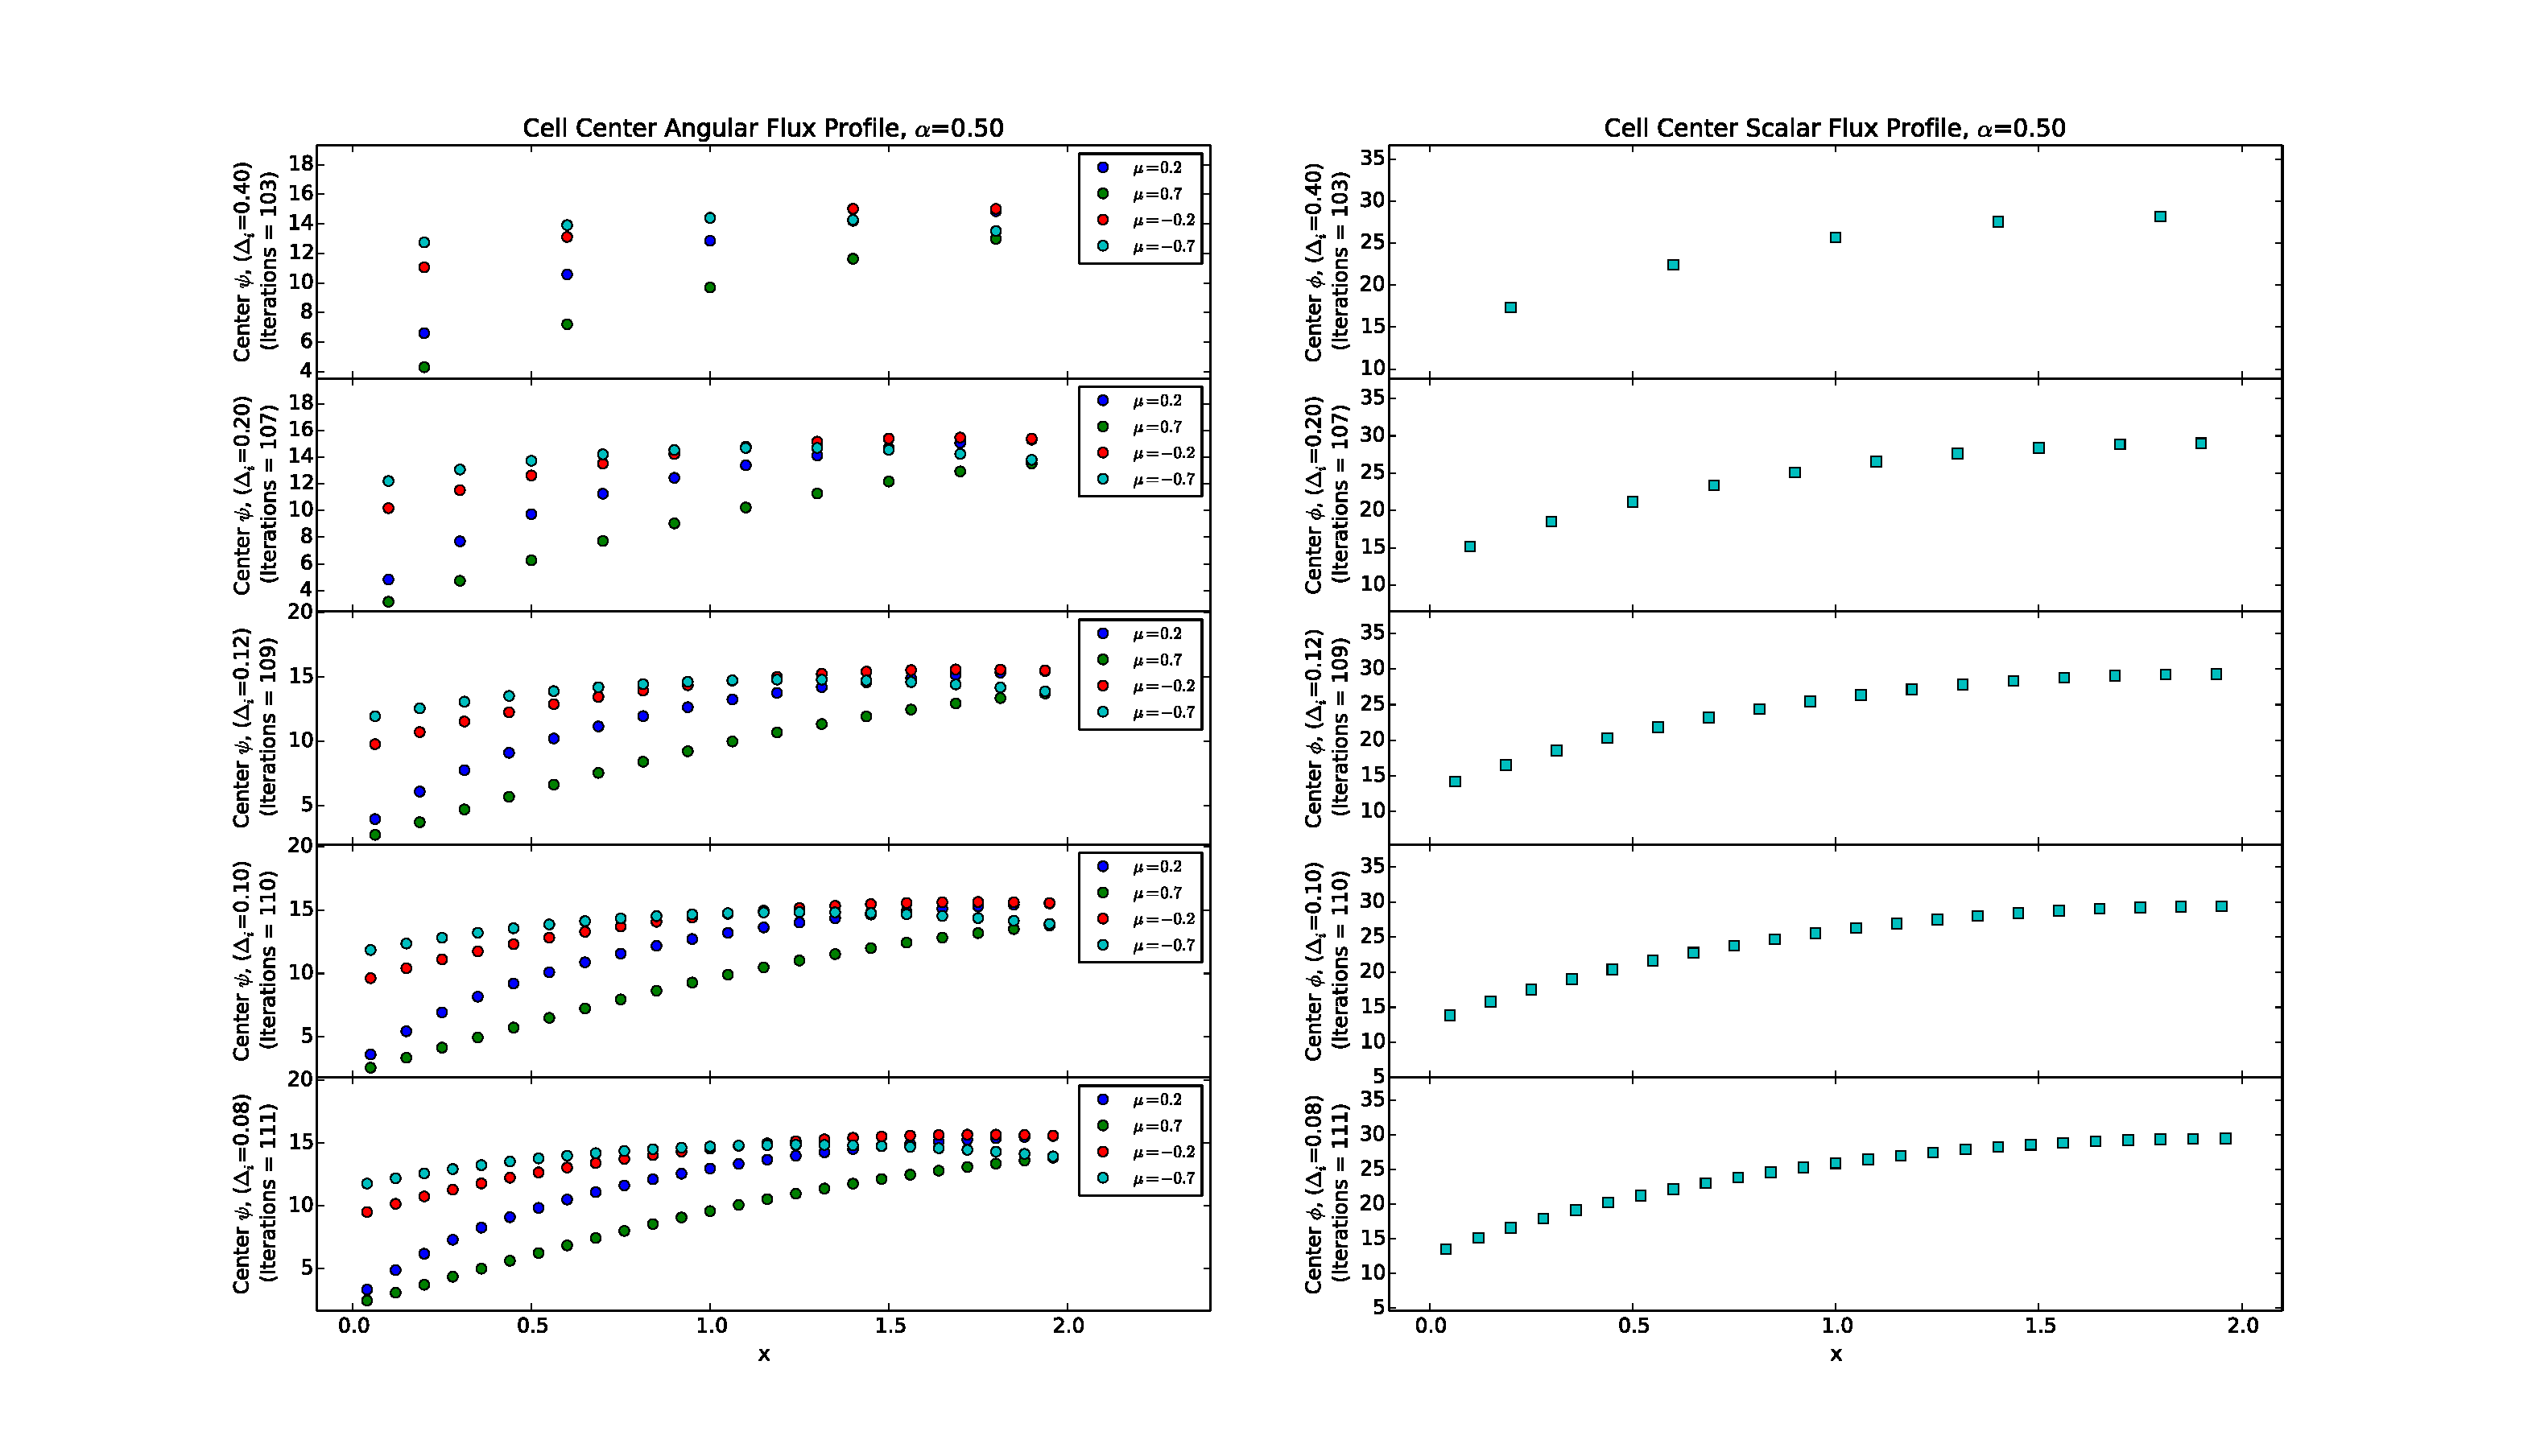
\includegraphics[width=0.9\textwidth]{Figures/FluxProfile_a=05_source}
    \caption{Center angular and scalar flux profiles for varying mesh spacings with $\alpha = 0.5$, with scattering ($\Sigma_s = 0.5$) and external source ($q_e=1$).}
    \label{fig10}
\end{figure}

\newpage
We see that the value of $\alpha$ did not make much of a difference in the results. But it did however have an effect on the required number of iterations before convergence (at least moving away from $\alpha = -0.5$).

%
%
%

\vspace{10pt}
\begin{enumerate}[(d)]
\item What happens with $\alpha = 0$ and $\Sigma_s = 0.9$?
\end{enumerate}

If we rerun the above code with these inputs, Python indicates that an overflow has occurred. If we profile the code a bit, we see that the flux keeps increasing with every iteration. The values eventually get larger than the declared variable type can handle, thus it reports an overflow. With scattering essentially being the only interaction ($\Sigma_s$ close to $\Sigma_t$), it seems we are unable to converge on a flux solution.





% - - - - - - - - - - - - - - - - - - - - - - - - - - - - - - - - - - - - - - - - - -
%\vspace{20pt}
\newpage
\noindent \textbf{Problem 4}\\
Starting from the following general system of equations
%
\begin{equation*}
\frac{\mu_a}{h_i}(\psi_{a,i+1/2}^g - \psi_{a,i-1/2}^g)+ \Sigma_{t,i}^g\psi_{a,i}^g = 2\pi\sum_{a=1}^N w_a \sum_{g'=1}^G \Sigma_{s, i}^{gg'}(a'\rightarrow a)\psi_{a',i}^{g'} + \frac{\chi_g}{2}\sum_{g'=1}^G \nu_{g'}\Sigma_{f,i}^{g'} \phi_{i}^{g'} + \frac{1}{2}Q_i^g\:,
\end{equation*}

where  $\phi$ \textit{is} scalar flux, write a set of five coupled equations for a five group problem. Assume neutrons can only downscatter from fast groups (1 and 2) to thermal groups (3, 4, and 5). Assume that thermal groups can upscatter into other thermal groups and can downscatter. Assume there is an external source and a fission source.\\

$\Rightarrow$ From the wording of the question, we assume the following about scattering: Neutrons in group 1 can downscatter to groups 3, 4, and 5. Neutrons in group 2 can downscatter into groups 3, 4, and 5. Neutrons in group 3 can downscatter into groups 4 and 5. Neutrons in group 4 can downscatter into group 5 and upscatter into group 3. Neutrons in group 5 can upscatter into groups 3 and 4. Neutrons in each group can also participate in in-group scattering ($3\rightarrow3$, $5\rightarrow5$, etc.). We also assume the following about fission: Neutrons can undergo fission in any group, and fission neutrons can be born into any group. Finally, we assume there is an external neutron source in every group. \\

%\begin{table}[htb]
%\centering
%\begin{tabular}{|c|c|c|c|c|}
%\hline
%Group & Where can neutrons scatter to? & Can fission occur? & Fission neutrons born here? & External Source? \\
%\hline
%1 & 1,3,4,5 & Yes & Yes & Yes \\
%2 & 2,3,4,5 & Yes & Yes & Yes \\
%3 & 3,4,5 & Yes & Yes & Yes \\
%4 & 3,4,5 & Yes & Yes & Yes \\
%5 & 3,4,5 & Yes & Yes & Yes \\
%\hline
%\end{tabular}
%\end{table}


\textbf{g = 1:}
\begin{align*}
\frac{\mu_a}{h_i}(\psi_{a,i+1/2}^1 - \psi_{a,i-1/2}^1)+ \Sigma_{t,i}^1\psi_{a,i}^1 = 2\pi\sum_{a=1}^N w_a \left[ \Sigma_{s, i}^{1\rightarrow1}(a'\rightarrow a)\psi_{a',i}^{1} \right] + \frac{\chi_1}{2} [ \nu_{1}\Sigma_{f,i}^{1}\phi_{i}^{1} + \nu_{2}\Sigma_{f,i}^{2}\phi_{i}^{2} + \nu_{3}\Sigma_{f,i}^{3}\phi_{i}^{3} \\ + \nu_{4}\Sigma_{f,i}^{4}\phi_{i}^{4} + \nu_{5}\Sigma_{f,i}^{5}\phi_{i}^{5} ] + \frac{1}{2}Q_i^1
\end{align*}

\textbf{g = 2:}
\begin{align*}
\frac{\mu_a}{h_i}(\psi_{a,i+1/2}^2 - \psi_{a,i-1/2}^2)+ \Sigma_{t,i}^2\psi_{a,i}^2 = 2\pi\sum_{a=1}^N w_a \left[ \Sigma_{s, i}^{2\rightarrow2}(a'\rightarrow a)\psi_{a',i}^{2} \right] + \frac{\chi_2}{2} [ \nu_{1}\Sigma_{f,i}^{1}\phi_{i}^{1} + \nu_{2}\Sigma_{f,i}^{2}\phi_{i}^{2}  + \nu_{3}\Sigma_{f,i}^{3}\phi_{i}^{3} \\ + \nu_{4}\Sigma_{f,i}^{4}\phi_{i}^{4} + \nu_{5}\Sigma_{f,i}^{5}\phi_{i}^{5} ] + \frac{1}{2}Q_i^2
\end{align*}

\textbf{g = 3:}
\begin{align*}
\frac{\mu_a}{h_i}(\psi_{a,i+1/2}^3 - \psi_{a,i-1/2}^3)+ \Sigma_{t,i}^3\psi_{a,i}^3 =  2\pi\sum_{a=1}^N w_a [ \Sigma_{s, i}^{1\rightarrow3}(a'\rightarrow a)\psi_{a',i}^{1} + \Sigma_{s, i}^{2\rightarrow3}(a'\rightarrow a)\psi_{a',i}^{2} + \Sigma_{s, i}^{3\rightarrow3}(a'\rightarrow a)\psi_{a',i}^{3} \\ + \Sigma_{s, i}^{4\rightarrow3}(a'\rightarrow a)\psi_{a',i}^{4} + \Sigma_{s, i}^{5\rightarrow3}(a'\rightarrow a)\psi_{a',i}^{5} ] + \frac{\chi_3}{2} [ \nu_{1}\Sigma_{f,i}^{1}\phi_{i}^{1} + \nu_{2}\Sigma_{f,i}^{2}\phi_{i}^{2} + \nu_{3}\Sigma_{f,i}^{3}\phi_{i}^{3} \\ + \nu_{4}\Sigma_{f,i}^{4}\phi_{i}^{4} + \nu_{5}\Sigma_{f,i}^{5}\phi_{i}^{5} ] + \frac{1}{2}Q_i^3
\end{align*}

\textbf{g = 4:}
\begin{align*}
\frac{\mu_a}{h_i}(\psi_{a,i+1/2}^4 - \psi_{a,i-1/2}^4)+ \Sigma_{t,i}^4\psi_{a,i}^4 =  2\pi\sum_{a=1}^N w_a [ \Sigma_{s, i}^{1\rightarrow4}(a'\rightarrow a)\psi_{a',i}^{1} + \Sigma_{s, i}^{2\rightarrow4}(a'\rightarrow a)\psi_{a',i}^{2} + \Sigma_{s, i}^{3\rightarrow4}(a'\rightarrow a)\psi_{a',i}^{3} \\ + \Sigma_{s, i}^{4\rightarrow4}(a'\rightarrow a)\psi_{a',i}^{4} + \Sigma_{s, i}^{5\rightarrow4}(a'\rightarrow a)\psi_{a',i}^{5} ] + \frac{\chi_4}{2} [ \nu_{1}\Sigma_{f,i}^{1}\phi_{i}^{1} + \nu_{2}\Sigma_{f,i}^{2}\phi_{i}^{2} + \nu_{3}\Sigma_{f,i}^{3}\phi_{i}^{3} \\ + \nu_{4}\Sigma_{f,i}^{4}\phi_{i}^{4} + \nu_{5}\Sigma_{f,i}^{5}\phi_{i}^{5} ] + \frac{1}{2}Q_i^4
\end{align*}

\textbf{g = 5:}
\begin{align*}
\frac{\mu_a}{h_i}(\psi_{a,i+1/2}^5 - \psi_{a,i-1/2}^5)+ \Sigma_{t,i}^5\psi_{a,i}^5 =  2\pi\sum_{a=1}^N w_a [ \Sigma_{s, i}^{1\rightarrow5}(a'\rightarrow a)\psi_{a',i}^{1} + \Sigma_{s, i}^{2\rightarrow5}(a'\rightarrow a)\psi_{a',i}^{2} + \Sigma_{s, i}^{3\rightarrow5}(a'\rightarrow a)\psi_{a',i}^{3} \\ + \Sigma_{s, i}^{4\rightarrow5}(a'\rightarrow a)\psi_{a',i}^{4} + \Sigma_{s, i}^{5\rightarrow5}(a'\rightarrow a)\psi_{a',i}^{5} ] + \frac{\chi_5}{2} [ \nu_{1}\Sigma_{f,i}^{1}\phi_{i}^{1} + \nu_{2}\Sigma_{f,i}^{2}\phi_{i}^{2} + \nu_{3}\Sigma_{f,i}^{3}\phi_{i}^{3} \\ + \nu_{4}\Sigma_{f,i}^{4}\phi_{i}^{4} + \nu_{5}\Sigma_{f,i}^{5}\phi_{i}^{5} ] + \frac{1}{2}Q_i^5
\end{align*}





% - - - - - - - - - - - - - - - - - - - - - - - - - - - - - - - - - - - - - - - - - -

\end{document}
